\documentclass[11pt]{amsart}

\usepackage{graphics}
\usepackage{graphicx}
%\usepackage{arxiv}
%\usepackage{enseign}
%\usepackage[utf8]{inputenc} % allow utf-8 input
\usepackage[T1]{fontenc}    % use 8-bit T1 fonts

\usepackage{amsthm}
\usepackage{amsbsy,amsmath,amssymb,amscd,amsfonts}
%\usepackage{biblatex}
%\addbibresource{elliptic_billiards_v2.bib}
%\usepackage[pagebackref=true]{hyperref}
\usepackage{hyperref}
\usepackage{url}            % simple URL typesetting
\usepackage{booktabs}       % professional-quality tables
\usepackage{nicefrac}       % compact symbols for 1/2, etc.
\usepackage{microtype}      % microtypography

\usepackage{float,latexsym,color}
%\usepackage{refcheck}
%\usepackage{mathspec}
\usepackage[font={scriptsize,it}]{caption}
\usepackage{subcaption}
%\let\proof\relax
%\let\endproof\relax
\usepackage{tablefootnote}

\usepackage{makecell}
\renewcommand{\arraystretch}{1.1}

\usepackage[dvipsnames]{xcolor}

\newtheorem{theorem}{Theorem}
\newtheorem{step}{Step}
\newtheorem{observation}{Observation}
\newtheorem{proposition}{Proposition}
\newtheorem{remark}{Remark}
\newtheorem{corollary}{Corollary}
\newtheorem{definition}{Definition}
\newtheorem{lemma}{Lemma}
\newtheorem*{lemma*}{Lemma}
\newtheorem{question}{Question}
\newtheorem{affirmation}{Affirmation}

\hypersetup{
    %bookmarks=true,         % show bookmarks bar?
    %unicode=true,          % non-Latin characters in Acrobat’s bookmarks
    pdftoolbar=true,        % show Acrobat’s toolbar?
    pdfmenubar=true,        % show Acrobat’s menu?
    pdffitwindow=false,     % window fit to page when opened
    pdfstartview={FitH},    % fits the width of 
    colorlinks=true,       % false: boxed links; true: colored links
    linkcolor=OliveGreen,          % color of internal links (change box color with linkbordercolor)
    citecolor=blue,        % color of links to bibliography
    filecolor=black,      % color of file links
    urlcolor=red           % color of external links
}

\usepackage{lineno}
\def\linenumberfont{\normalfont\small\sffamily}
%a4: 210 x 297
%\textwidth=125mm
%\textheight=195mm
\arraycolsep=2pt
\captionsetup{width=120mm}

\DeclareMathOperator*{\argmin}{arg\,min} % thin space, limits underneath in displays

\newcommand{\torp}[2]{\texorpdfstring{#1}{#2}}

\title[3-periodics: why so many ellipses?]{Loci of 3-periodics in an Elliptic Billiard:\\Why so many ellipses?}

\author{Ronaldo Garcia}
\address{Ronaldo Garcia\\
Inst. de Matemática e Estatística\\
Univ. Federal de Goiás\\
Goiânia, GO, Brazil}
\email{ragarcia@ufg.br}

\author{Dan Reznik}
\address{Dan Reznik\\
Data Science Consulting\\
Rio de Janeiro, RJ, Brazil}
\email{dan@dat-sci.com}

\author{Jair Koiller}
\address{Jair Koiller\\
Dept. de Matemática\\
Univ. Federal de Juiz de Fora\\
Juiz de Fora, MG, Brazil}
\email{jairkoiller@gmail.com}

\begin{document}

\begin{abstract}
A triangle center such as the incenter, barycenter, etc., is specified by function on sidelengths and/or angles. Consider the 1d family of 3-periodics in the elliptic billiard, and the loci of its triangle centers. Some will sweep ellipses, others quartics, sextics, etc. We propose two rigorous methods to prove if the locus of a given center is an ellipse. The first one is based on computer algebra, and the second one on the Theory of Resultants, which yields an implicit two-variable polynomial whose zero set contains the locus. We also prove that if the triangle center function is rational on sidelengths, the locus is algebraic.\\

\noindent \textbf{Keywords}: elliptic billiard, periodic trajectories, triangle center, derived triangle, locus, loci, algebraic.\\

\noindent \textbf{MSC2010} {37-40 \and 51N20 \and 51M04 \and 51-04}

\end{abstract}

 
 
%\setpagewiselinenumbers
\modulolinenumbers[1]
%\linenumbers

\maketitle

\section{Introduction}
\label{sec:intro}
Classic {\em triangle centers} such as the incenter, barycenter, etc., are traditionally obtained via simple geometric constructions. Indeed, these can also be specified by special {\em triangle functions} which operate cyclically on sidelengths and/or angles \cite{kimberling1993_rocky}; see Appendix~\ref{app:triangle-centers}. Thousands appear on Kimberling's Encyclopedia  \cite{etc}. The list includes triangle functions which are rational, irrational, and more rarely, transcendental on sidelengths and/or angles. 

Consider the 1d family of 3-periodic orbits in the elliptic billiard (EB), Figure~\ref{fig:3-periodics}. The vertices are bisected by ellipse normals and the sides are tangent to a virtual confocal caustic; see Appendix~\ref{app:billiards} for a review. We have been drawn to this family because unexpectedly, the locus of the incenter is an ellipse and that of the {\em Mittenpunkt} $X_9$\footnote{The $X_k$ notation is after Kimberling \cite{etc}. The Mittenpunkt, was discovered by Nagel in 1836 as the point of concurrence of lines from the excenters through side midpoints \cite{mw}.} is the billiard center \cite{reznik2020-intelligencer}. Additionally, many other curious invariants have been detected and/or proved \cite{akopyan2020-invariants,bialy2020-invariants,reznik2020-invariants}. 

\begin{figure}
    \centering
    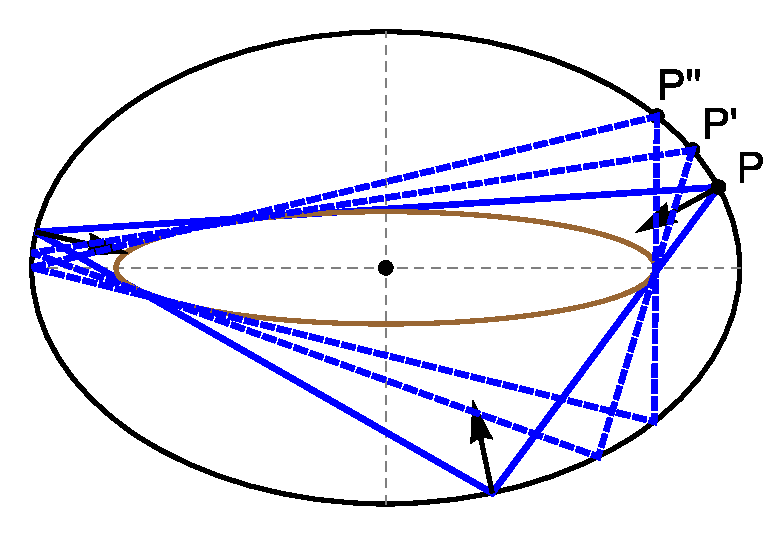
\includegraphics[width=.5\textwidth]{pics_1005_three_orbits_proofs.eps}
    \caption{Three 3-periodic orbits (one solid with vertex $P$ and two dashed with vertices $P'$, $P''$). The vertices are bisected by ellipse normals and the sides are dynamically tangent to a virtual confocal caustic (brown). Remarkably, the family conserves perimeter \cite{sergei91}. \href{https://bit.ly/38oncCD}{app}}
    \label{fig:3-periodics}
\end{figure}

In general, triangle centers sweep such curves as ellipses, quartics, sextics, etc., with or without self-intersections, etc.; see Figure~\ref{fig:incenter-loci}. The central question here is: given a triangle center, is it possible to predict its locus curve type over billiard 3-periodics based on the triangle function?

\begin{figure}
    \centering
    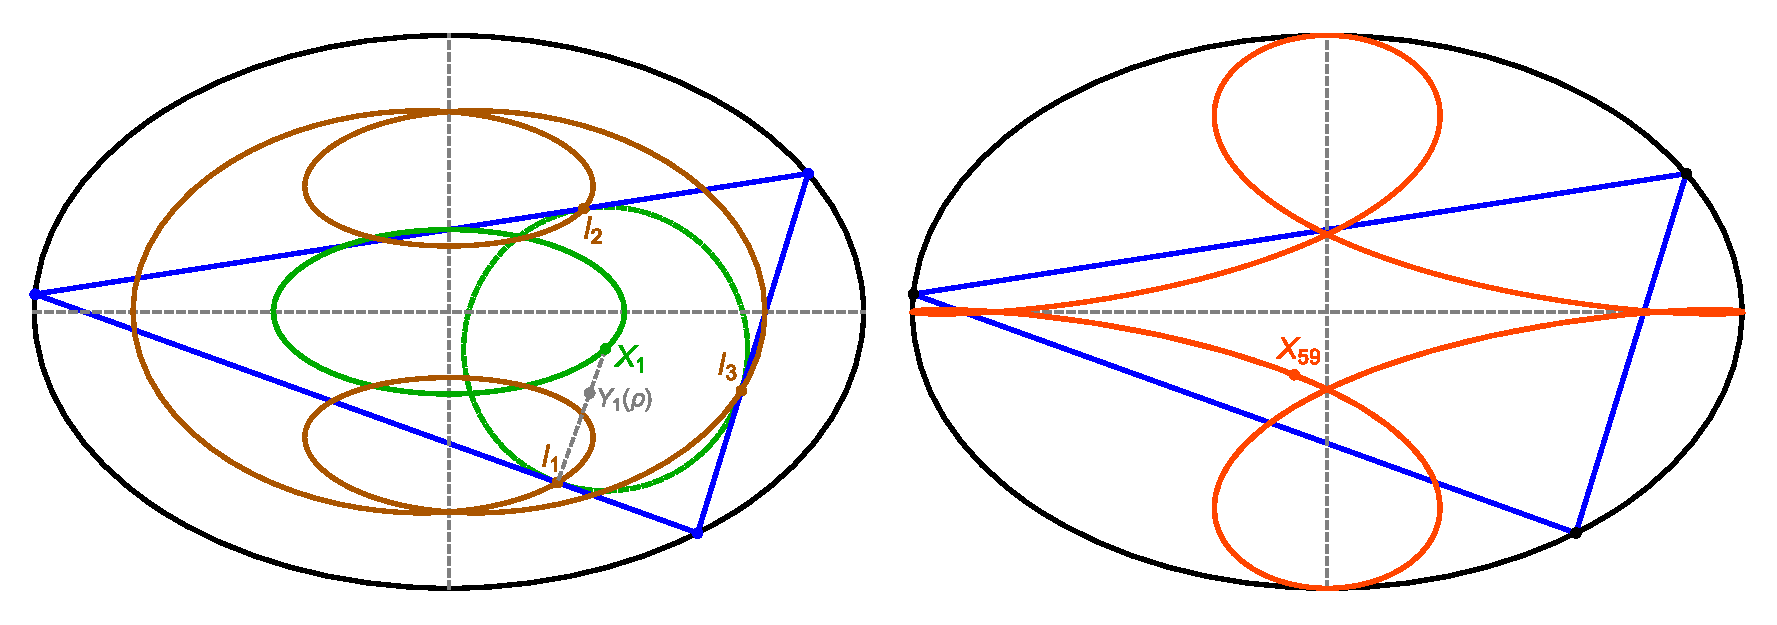
\includegraphics[width=\textwidth]{pics_1021_x1_x59}
    \caption{\textbf{Left}: A sample 3-periodic orbit (blue), the elliptic locus of the Incenter $X_1$ (green) and of that of the Intouchpoints $I_1,I_2,I_3$ (brown), the points of contact of the Incircle (dashed green) with the orbit sides. These produce a curve with two internal lobes whose degree is at least 6. $Y_1(\rho)$ is a convex combination of $X_1$ and $I_1$ referred to in Section~\ref{sec:triple-winding}. \href{https://bit.ly/3q4b0Nn}{app},  \href{https://youtu.be/BBsyM7RnswA}{Video 1}, \href{https://youtu.be/9xU6T7hQMzs}{Video 2}. \textbf{Right}: The locus of $X_{59}$ is a curve with four self-intersections. A vertical line epsilon away from the origin intersects the locus at 6 points. \href{https://bit.ly/3i4h6dX}{app}}
    \label{fig:incenter-loci}
\end{figure}

\subsection*{Main Results}

We present a method to rigorously verify if the locus of given triangle center is an ellipse or not. We apply it to the first 100 Centers listed in \cite{etc}, finding that 29 are elliptic. We have derived explicit expressions for their axes \cite{garcia2021-ellipses-web}.

We prove (Theorem~\ref{thm:rational-center}) that when a triangle center is rational on the sidelengths, the locus (elliptic or not) will be algebraic. We also describe a method based on the theory of resultants which computes the irreducible polynomial in two variables, whose zero set is the Zariski Closure \cite{cox2005-AG} of the locus. From wide experimentation, no irrational triangle function has yet produced an elliptic locus, so it is likely that for a locus to be elliptic its triangle function must be rational.

We also consider the curious case of the Symmedian Point $X_6$, whose locus closely approximates an ellipse but it is actually a quartic, which we derive explicitly. Interestingly, its triangle function is rational and one of the simplest in \cite{etc}; see Table~\ref{tab:center-trilinears}.

For the general case of triangle function to locus type, we still lack a theory.

\subsection*{Related Work}

Odehnal extensively studied loci of triangle centers over the poristic triangle family \cite{odehnal2011-poristic}. Our early experimental result that the locus of the Incenter $X_1$ of billiard 3-periodics is an ellipse was subsequently proven \cite{olga14,garcia2019-incenter}. Proofs soon followed for the ellipticity of both $X_2$ \cite{sergei2016-com} and $X_3$ \cite{corentin19,garcia2019-incenter}; see Figures \ref{fig:non-elliptic-vertex} and \ref{fig:x12345-feuer-combo} in Appendix~\ref{app:early}.

\subsection*{Outline}

Our main methods appear in Sections~\ref{sec:loci_geom} and \ref{sec:algebraic}. We conclude in Section~\ref{sec:conclusion} with a list of questions and interesting links and videos. The Appendices contain supporting material. Most figures contain clickable links to relevant videos and/or the experiment displayed on our browser-based \href{https://dan-reznik.github.io/ellipse-mounted-loci-p5js}{app} \cite{darlan2020-ellipse-mounted}.


\section{Detecting Elliptic Loci}
\label{sec:loci_geom}
Let the boundary of the EB be given by ($a>b>0$):
\begin{equation}
f(x,y)=\left(\frac{x}{a}\right)^2+\left(\frac{y}{b}\right)^2=1.
\label{eqn:billiard-f}
\end{equation}

We describe a numerically-assisted method\footnote{We started with visual inspection, but this is both laborious and unreliable, some loci (take $X_{30}$ and $X_6$ as examples) are indistinguishable from ellipses to the naked eye.} which proves that the locus of a given Triangular Center is elliptic or otherwise. We then apply it to the first 100 Triangle Centers\footnote{An arbitrarily large list can be tested.} listed in \cite{etc}.

\subsection{Proof Method}

Our proof method consists of two phases, one numeric, and one symbolic, Figure~\ref{fig:method-pipeline}. It makes use of the following Lemmas, whose proofs appear in Appendix~\ref{app:method-lemmas}:

\begin{lemma}
The locus of a Triangle Center $X_i$ is symmetric about both EB axes and centered on the latter's origin.
\label{lem:axisymmetric}
\end{lemma}

\begin{proof} 
Given a 3-periodic $T=P_1P_2P_3$. Since the EB is symmetric about its axes, the family will contain the reflection of $T$ about said axes, call these $T'$ and $T''$. Since Triangle Centers are invariant with respect to reflections, Appendix~\ref{app:triangle-centers}, $X_i'$ and $X_i''$ will be found at similary reflected locations.
\end{proof}

Note that  if the locus is elliptic, the above implies it will be concentric and axis-aligned with the EB.

%\begin{lemma}
%\label{lem:axisymmetric}
%The locus of a Triangle Center $X_i$ is symmetric about both EB axes and centered on the latter's origin.
%\end{lemma}

%\begin{proof} Let $X_i =(c_i,d_i)$ be a triangular center of the billiard orbit $P_1=(x_1,y_1), P_2=(x_2,y_2), P_3=(x_3,y_3)$. For the reflections $\pi_1(x,y)=(x,-y)$,   $\pi_2(x,y)=(-x,y)$ and antipodal $\pi_3(x,y)=-(x,y)$ the triangles $Q_1=\pi_j(P_1), Q_2=\pi_j(P_2), Q_3=\pi_j(P_3)$, ($j=1,2,3$), are also   billiard orbits, and by equation \eqref{eqn:trilin-cartesian} its triangular center is $Y_i=\pi_j(X_i). $  This ends the proof.
%
%\end{proof}

\begin{lemma}
\label{lem:axis-of-symmetry}
Any Triangle Center $X_i$ of an isosceles triangle is on the axis of symmetry of said triangle.
\end{lemma}

\begin{lemma}
\label{lem:center-cover}
A parametric traversal of $P_1$ around the EB boundary triple covers the locus of Triangle Center $X_i$, elliptic or not.
\end{lemma}

See Section~\ref{sec:triple-winding} for more details.

A first phase fits a concentric, axis-aligned ellipse to a fine sampling of the locus of some Triangle Center $X_i$. A good fit occurs when the error is several orders of magnitude\footnote{Robust fitting of ellipses to a cloud of points is not new \cite{fitzgibbon99-ellipse}. In our case, the only source of error in Triangle Center coordinates is numerical precision, whose propagation can be bounded by Interval Analysis \cite{moore2009-interval-analysis,snyder92-ellipse}.} less than the sum of axes regressed by the process. False negatives are eliminated by setting the error threshold to numeric precision. False positives can be produced by adding arbitrarily small noise to samples of a perfect ellipse, though this type of misclassification does not survive the next, symbolic phase. 

A second phase attempts to symbolically verify via a Computer Algebra System (CAS) if the parametric locus of the $X_i$ satisfies the equation of a concentric, axis-aligned ellipse. Expressions for its semi-axes are obtained by evaluating $X_i$ at isosceles orbit configurations, Figure~\ref{fig:sideways-upright-orbit}. The method is explained in detail in Figure~\ref{fig:method-detail}.

\begin{figure}
    \centering
    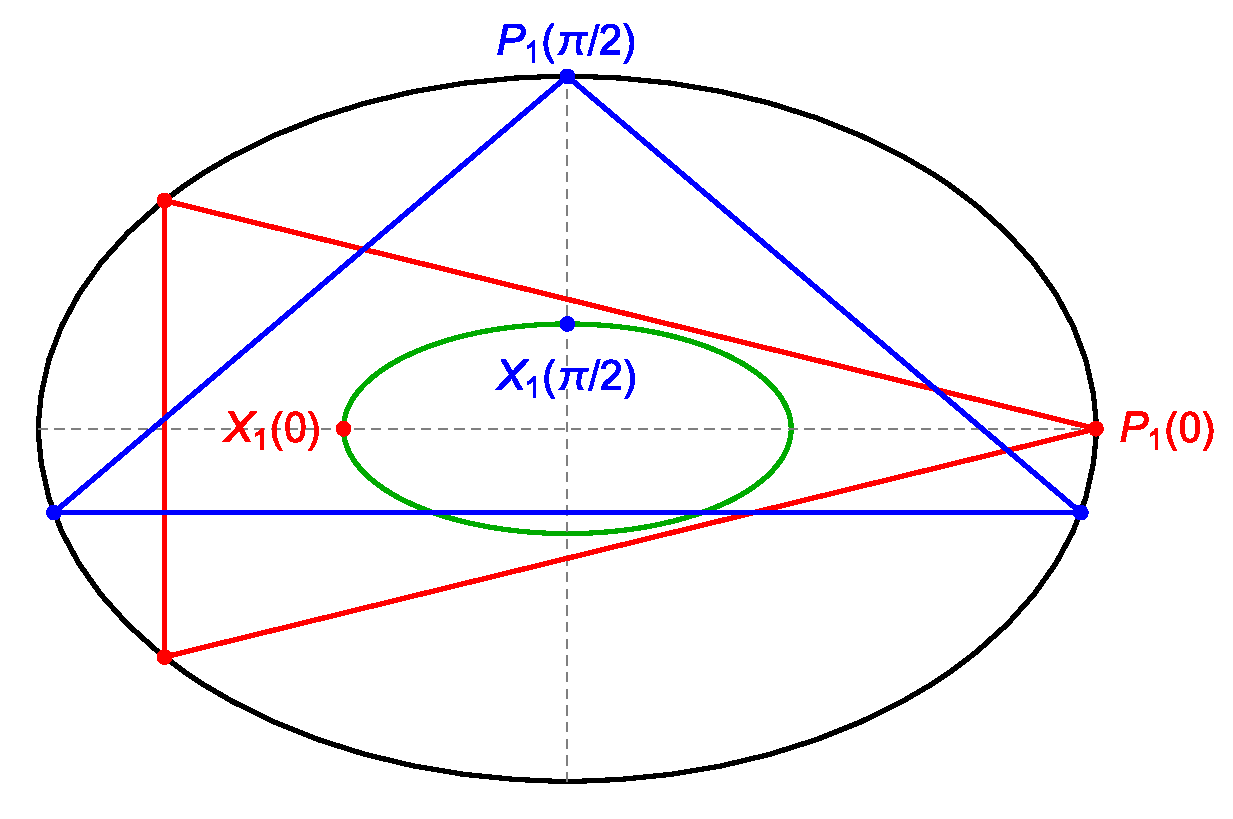
\includegraphics[width=.5\textwidth]{pics_1060_two_isosceles}
    \caption{With $P_1$ at the right (resp.~top) vertex of the EB, the orbit is a sideways (resp.~upright) isosceles triangle, solid red (resp.~solid blue). Not shown are their two symmetric reflections. Also shown (green) is the locus of a sample Triangle Center, $X_1$ in this case. At the isosceles positions, vertices will lie on the axis of symmetry of the triangle, Lemma~\ref{lem:axis-of-symmetry}. When the locus is elliptic, the $x,y$ coordinates of $X_i(0),X_i(\pi/2)$ are the semi-axes $a_i,b_i$, respectively.}
    \label{fig:sideways-upright-orbit}
\end{figure}

\begin{figure}
    \centering
    %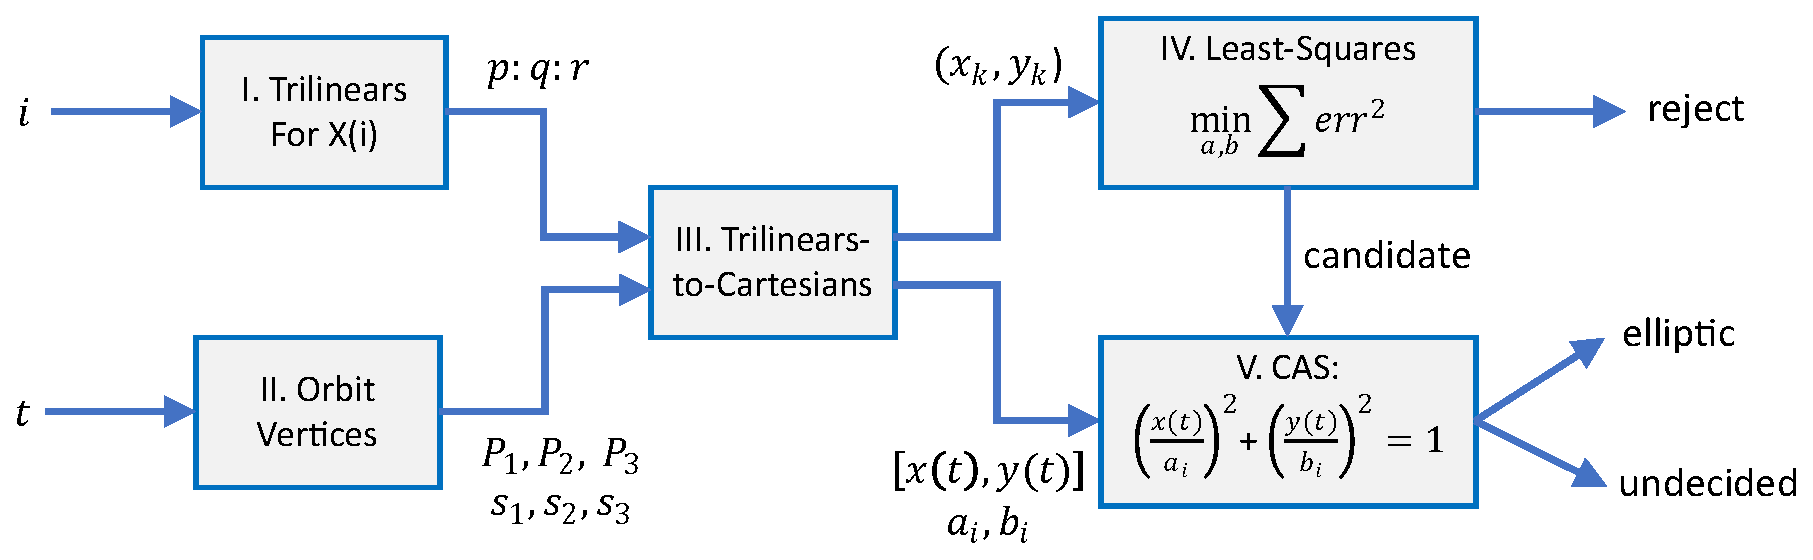
\includegraphics[trim={0 7.5cm 0 1cm},clip,width=\textwidth]{pics_1130_algo_proof_elliptic.eps}
    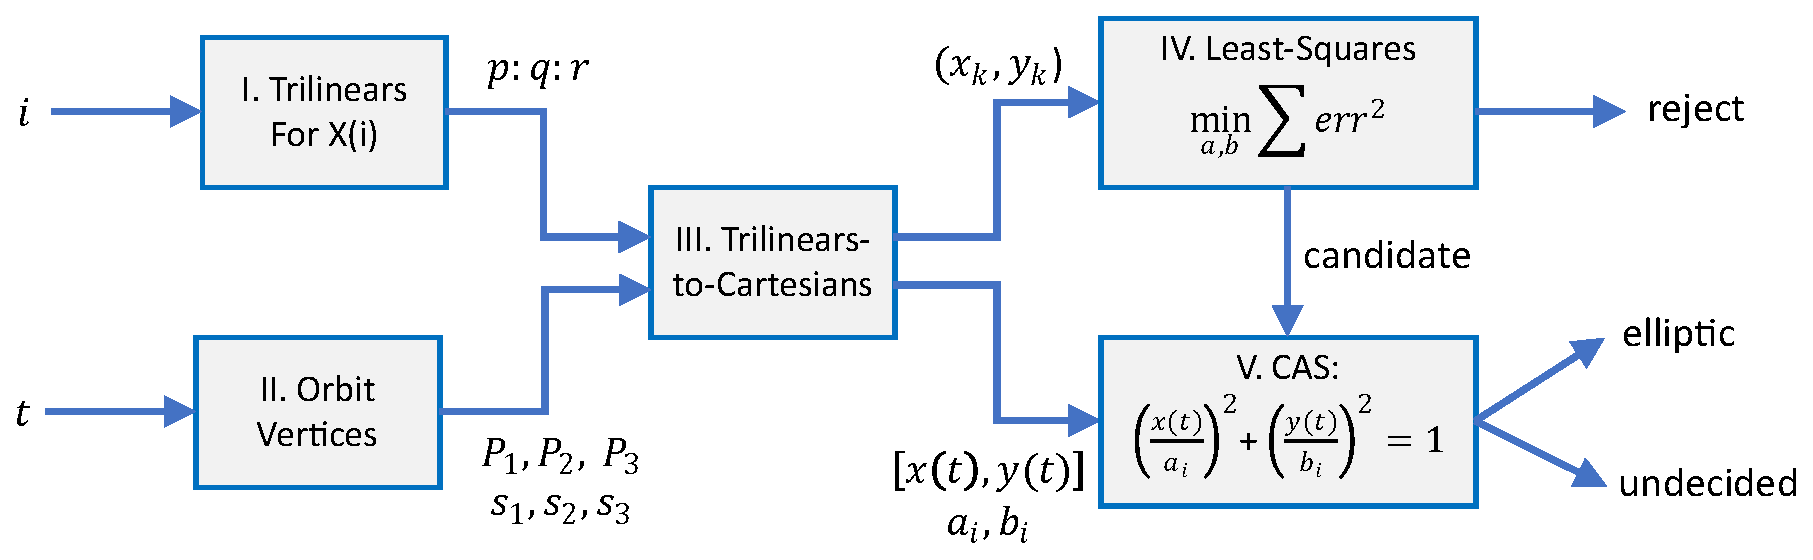
\includegraphics[width=.9\textwidth]{pics_1130_algo_proof_elliptic.eps}
    \caption{Our method as a flow-chart, modules labeled from I to V: (I) The ith center is specified and its Trilinears $p:q:r$ are obtained from ETC \cite{etc}. (II) Given a symbolic parameter $t$ or a numeric sample $t_k$, obtain Cartesians for orbit vertices and the sidelengths, Appendix~\ref{app:p1p2p3}. (III) Combine Trilinears and orbit data to obtain, via \eqref{eqn:trilin-cartesian}, numeric Cartesians for $X_i(t_k)$ or symbolically as $X_i(t)$. (IV) Least-squares fit an axis-aligned, concentric ellipse to the $(x_k,y_k)$ samples and accept $X_i$ as candidate if the fit error is sufficiently small. (V) Verify, via a Computer Algebra System (CAS), if the parametric locus $X_i(t)$ satisfies the equation of an ellipse whose axes $a_i,b_i$ are obtained symbolically in II-III by setting $t=0,\pi/2$. If the CAS is successful, $X_i(t)$ is deemed elliptic, otherwise the result is ``undecided''. The CAS was successful for all 29 candidates selected by IV out of the first 100 Kimberling Centers.}
    \label{fig:method-pipeline}
\end{figure}

% The philosophy: 

%In the quest to determine  elliptic loci, an human observer could discard, visually,  plots having loops and/or that are non convex.  However, it could be quite a different story   to distinguish a (true)  ellipse from a symmetric oval, just visually, as the plots of   $X_6$  and $X_?$ exemplify.   This  task is outside our realm - it may belong to neuroperception. Architects and painters do have a keen eye but even so there is a limit to their abilities \cite{Ochkov2019}, \cite{Xing2018}, \cite{Duvernoy2015}, \cite{Mazzotti2017}. 

%Hence we  opted to avoid   direct human involvement. The ideia is to  work  as much as possible in an automated fashion.  

%Pattern recognition algorithms for ellido exist, but they are costly. Moreover, we feared %that could be  prone to false positives or negatives. 

%The screening procedure:

% \subsection{Outline of the two steps}
\begin{figure}
\fbox{
\begin{minipage}{\textwidth}
\footnotesize
\noindent \textbf{1. Select Candidates:}
\begin{itemize}
\item Let the EB have axes $a,b$ such that $a>b>0$. Calculate $P_1(t_k)=\left(a\cos(t_k),b\sin(t_k)\right)$, for $M$ equally-spaced samples $t_k\in[0,2\pi)$, $k=1,2,...,M$.
\item Obtain the Cartesian coordinates for the orbit vertices $P_2(t_k)$ and $P_3(t_k)$, $\forall k$ (Appendix~\ref{app:p1p2p3}).
\item Obtain the Cartesians for Triangle Center $X_i$ from its Trilinears \eqref{eqn:trilin-cartesian}, for $\forall{t_k}$. If analyzing the vertex of a Derived Triangle, convert a row of its {\em Trilinear Matrix} to Cartesians, Appendix~\ref{app:derived-tris}.
\item Least-squares fit an origin-centered, axis-aligned ellipse (2 parameters) to the $X_i(t_k)$ samples, Lemma~\ref{lem:axisymmetric}. Accept the locus as potentially elliptic if the numeric fit error is negligible, rejecting it otherwise.
\end{itemize}
\noindent \textbf{2. Verify with CAS}
\begin{itemize}
    \item Taking $a,b$ as symbolic variables, calculate $X_i(0)$ (resp.~$X(\pi/2)$), placing $P_1$ at the right (resp.~top) EB vertex. The orbit will be a sideways (resp.~upright) isosceles triangle, Figure~\ref{fig:sideways-upright-orbit}. By Lemma~\ref{lem:axis-of-symmetry}, $X_i$ will fall along the axis of symmetry of either isosceles.
    \item The $x$ coordinate of $X_i(0)$ (resp.~the $y$ of  $X_i(\pi/2)$) will be symbolic expressions in $a,b$. Use them as candidate locus semiaxes' lengths $a_i,b_i$.
    \item Taking $t$ as a symbolic variable, use a computer algebra system (CAS) to verify if $X_i(t)=\left(x_i(t),y_i(t)\right)$, as parametrics on $t$, satisfy $(x_i(t)/a_i)^2+(y_i(t)/b_i)^2=1$, ${\forall}t$.
    \item If the CAS is successful, Lemma~\ref{lem:center-cover} guarantees $X_i(t)$ is will cover the entire ellipse, so assert that the locus of $X_i$ is an ellipse. Else, locus ellipticity is indeterminate. 
\end{itemize}
\end{minipage}}
\caption{Method for detecting ellipticity of a Triangle Center locus.}
\label{fig:method-detail}
\end{figure}

\subsection{Phase 1: Least-Squares-Based Candidate Selection}

Let the position of $X_i(t)$ be sampled\footnote{Randomly or in equal intervals.} at $t_k\in[0,2\pi]$, $k=1{\ldots}M$. If the locus is an ellipse, than the latter is concentric and axis-aligned with the EB, Lemma~\ref{lem:axisymmetric}. Express the squared error as the sum of squared sample deviations from an implicit ellipse:

\begin{equation}
\text{err}^2(a_i,b_i)= \sum_{k=1}^M{\left[\left(\frac{x_k}{a_i}\right)^2+\left(\frac{y_k}{b_i}\right)^2-1\right]^2}
\label{eqn:fit-error}
\end{equation}

\noindent Least-squares can be used to estimate the semi-axes:

$$
(\hat{a_i},\hat{b_i})=\argmin_{a,b}\left\{ \text{err}^2(a_i,b_i)\right\}
$$

The first 100 Kimberling centers separate into two distinct clusters: 29 with negligible least-squares error, and 71 with finite ones. These are shown in ascending order of error in our companion website \cite[Part II]{garcia2021-ellipses-web}.

A gallery of loci generated by $X_1$ to $X_{100}$ (as well as vertices of several derived triangles) is provided in \cite{dsr_locus_gallery_2019}.

\subsection{Phase 2: Symbolic Verification with a CAS}

A CAS was successful in symbolically verifying that all 29 candidates selected in Phase 1 satisfy the equation of an ellipse (none were undecided). As an intermediate step, explicit expressions for their elliptic semi-axes were computed and appear in \cite[Part I]{garcia2021-ellipses-web}.

\begin{theorem} \label{main}
Out of the first 100 centers in \cite{etc}, exactly 29 produce elliptic loci, all of which are concentric and axis-aligned with the EB. These are $X_i$,i=1, 2, 3, 4, 5, 7, 8, 10, 11, 12, 20, 21, 35, 36, 40, 46, 55, 57, 63, 65, 72, 78, 79, 80, 84, 88, 90. Specifically:
\begin{itemize}
\item The loci of $X_i,i=2,7,57,63$ are ellipses similar to the EB.
\item The loci of $X_i,i=4,10,40$ are ellipses similar to a $90^\circ$-rotated copy of the EB.
\item The loci of $X_i,i=88,100$ are ellipses identical to the EB\footnote{See below for more centers on the EB discovered by Peter Moses and Deko Dekov.}.
\item The loci of $X_{55}$ is an ellipse similar to the $N=3$ Caustic.
\item The loci of $X_i,i=3,84$ are ellipses similar to a $90^\circ$-rotated copy of the $N=3$ Caustic.
\item The locus of $X_{11}$ is an ellipse identical to the $N=3$ Caustic.
\end{itemize}
\label{thm:loci29}
\end{theorem}

The properties above are summarized on Table~\ref{tab:ell}. Explicit expressions for the semi-axes in terms of $a,b$ for the above appear in \cite[Part I]{garcia2021-ellipses-web}. 

\begin{figure}
    \centering
    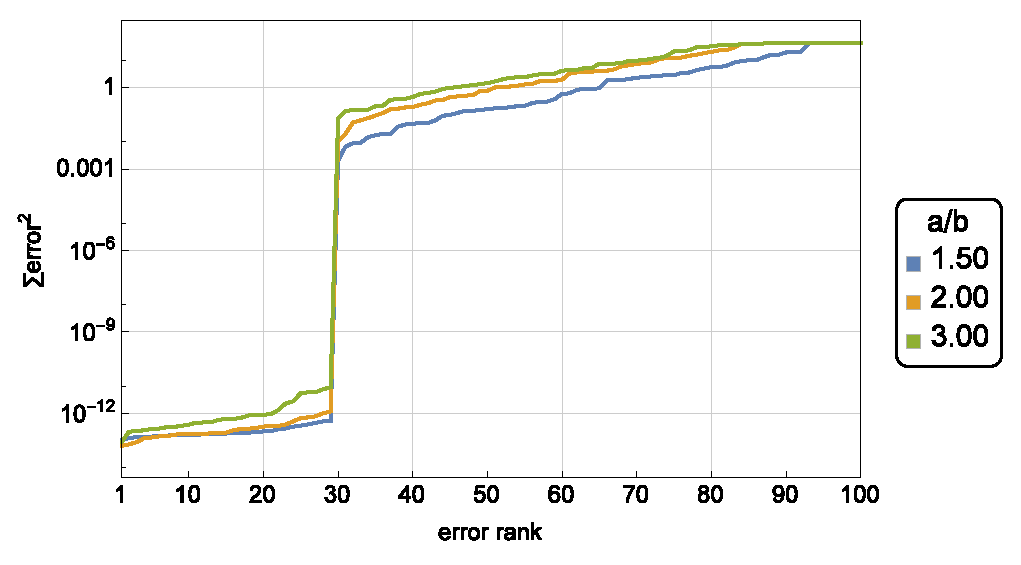
\includegraphics[width=.7\textwidth]{pics_1100_least_squares_error.eps}
    \caption{Log of Least-squares error for first 100 Kimberling centers in ascending order of error, for three values of $a/b$, $M=1500$. Elliptic vs. non-elliptic centers are clearly separated in two groups whose errors differ by several orders of magnitude. A table in \cite[Part II]{garcia2021-ellipses-web} shows that $X_{37}$ and $X_6$ are have ranks $30$ and $31$ respectively, i.e., they are the Centers whose non-elliptic loci are closest to a perfect ellipse.}
    \label{fig:least-squares-error-graph}
\end{figure}

\begin{table}
%\renewcommand{\arraystretch}{1.}
\begin{minipage}[t]{.475\linewidth}
$$
\scriptsize
\begin{array}{|c|c|l|c|}
\hline
\text{row} & X_i & \text{definition} & \text{sim} \\
\hline
 1 & {1} & \text{Incenter} & \text{J}^t \\
 2 & {2} & \text{Centroid} & \text{B} \\
 3 & {3} & \text{Circumcenter} & \text{C}^t  \\
 4 & {4} & \text{Orthocenter} & \text{B}^t \\
 5 & {5} & \text{9-Point Center} &  \\
 6 & {7} & \text{Gergonne Point} & \text{B}\\
 7 & {8} & \text{Nagel Point} &  \\
 8 & {10} & \text{Spieker Center} & \text{B}^t\\
 9 & {11} & \text{Feuerbach Point} & \text{C}^+ \\
 10 & {12} & \text{$\{X_{1,5}\}$-Harm.Conj. of $X_{11}$} & \\
 11 & {20} & \text{de Longchamps Point} & \\
 12 & {21} & \text{Schiffler Point} & \\
 13 & {35} & \text{$\{X_{1,3}\}$-Harm.Conj. of $X_{36}$} & \\
 14 & {36} & \text{Inverse-in-Circumc. of $X_1$} & \\
 15 & {40} & \text{Bevan Point} & \text{B}^t \\
 \hline
\end{array}
$$
\end{minipage}%
\begin{minipage}[t]{.475\linewidth}
$$
\scriptsize
\begin{array}{|c|c|l|c|}
\hline
\text{row} & X_i & \text{definition} & \text{sim} \\
\hline
16 & {46} & \text{$X_4$-Ceva Conj. of $X_1$} & \\
 17 & {55} & \text{Insimilictr(Circumc.,Incir.)} & \text{C}\\
 18 & {56} & \text{Exsimilictr(Circumc.,Incir.)} &  \\
 19 & {57} & \text{Isogonal Conj. of $X_9$} & \text{B} \\
 20 & {63} & \text{Isogonal Conj. of $X_{19}$} & \text{B} \\
 21 & {65} & \text{Intouch Triangle's $X_4$} & \\
 22 & {72} & \text{Isogonal Conj. of $X_{28}$} & \text{J}\\
 23 & {78} & \text{Isogonal Conj. of $X_{34}$} & \\
 24 & {79} & \text{Isogonal Conj. of $X_{35}$} & \\
 25 & {80} & \text{Refl. of $X_1$ about $X_{11}$} &  \text{J}^t \\
 26 & {84} & \text{Isogonal Conj. of $X_{40}$} & C^t \\
 27 & {88} & \text{Isogonal Conj. of $X_{44}$} &  \text{B}^+ \\
 28 & {90} & \text{$X_{3}$-Cross Conj. of $X_{1}$} & \\
 29 & {100} & \text{Anticomplement of $X_{11}$} & \text{B}^+\\
 \hline
 \end{array}
 $$
\end{minipage}
\caption{The 29 Kimberling centers within $X_1$ to $X_{100}$ with elliptic loci. Under column ``sim.'', letters B,C,J indicate the locus is similar to EB, Caustic, or Excentral locus, respectively. An additional {+}  (resp. {t}) exponent indicates the locus is identical (resp. similar to a perpendicular copy) to the indicated ellipse. Note: the ellipticity of  $X_i$,$i=1,2,3,4$ was previously proven \cite{olga14,sergei2016proj,corentin19,garcia2019-incenter}.}
\label{tab:ell}
\end{table}

\subsection{The quartic locus of the Symmedian Point}
\label{sec:symmedian}

At $a/b=1.5$ the locus of $X_6$, the Symmedian Point, is visually indistinguishable from an ellipse, Figure~\ref{fig:symmedian}. Fortunately, its fit error is 10 orders of magnitude higher than the ones produced by true elliptic loci, see \cite[Part II]{garcia2021-ellipses-web}. So it is easily rejected by the least-squares phase. Indeed, symbolic manipulation yields:

\begin{theorem}
 The locus of $X_6$ is a convex quartic given by:

\begin{equation*}
  \mathcal{X}_6(x,y)=c_1 x^4+c_2 y^4+c_3 x^2 y^2+ c_4 x^2 + c_5 y^2 = 0
\end{equation*}

\noindent where:
$$
\begin{array}{rlrl}
c_1=&b^4(5\delta^2-4(a^2-b^2)\delta -a^2 b^2)&c_2=&a^4(5\delta^2+4(a^2-b^2)\delta-a^2b^2) \\
c_3=&2a^2 b^2(a^2 b^2+3\delta^2)&c_4=&a^2 b^4(3 b^4+2(2 a^2-b^2)\delta-5\delta^2)\\
c_5=&a^4 b^2(3 a^4+2(2 b^2-a^2)\delta-5\delta^2)&\delta=&\sqrt{a^4-a^2 b^2+b^4}
\end{array}
$$
\end{theorem}

\begin{proof}
Using a CAS, obtain symbolic expressions for the coefficients of a quartic symmetric about both axes (no odd-degree terms), passing through 5 known-points. Still using a CAS, verify the symbolic parametric for the locus satisfies the quartic.
\end{proof}

 \noindent Note the above is also satisfied by a degenerate level curve $(x,y)=(0,0)$, which we ignore.

\begin{remark}
The axis-aligned ellipse $\mathcal{E}_6$ with semi-axes $a_6,b_6$ is internally tangent to $\mathcal{X}_6(x,y)=0$ at the four vertices where:
{\small  
\begin{align}
%a_6=&\frac{\left[(3\,a^2-b^2)\delta %-(a^2+b^2)b^2\right]a}{a^4+b^4+2\delta^2}\nonumber\\
a_6= \frac{\left[(3\,a^2-b^2)\delta -(a^2+b^2)b^2\right]a}{a^2b^2+3\delta^2},\;\;\;
b_6= \frac{\left[(a^2-3\,b^2)\delta + (a^2+b^2)a^2\right]b}{a^2b^2+3\delta^2}
\label{eqn:x6-ellipse}
\end{align}
}
\end{remark}

\begin{figure}
    \centering
    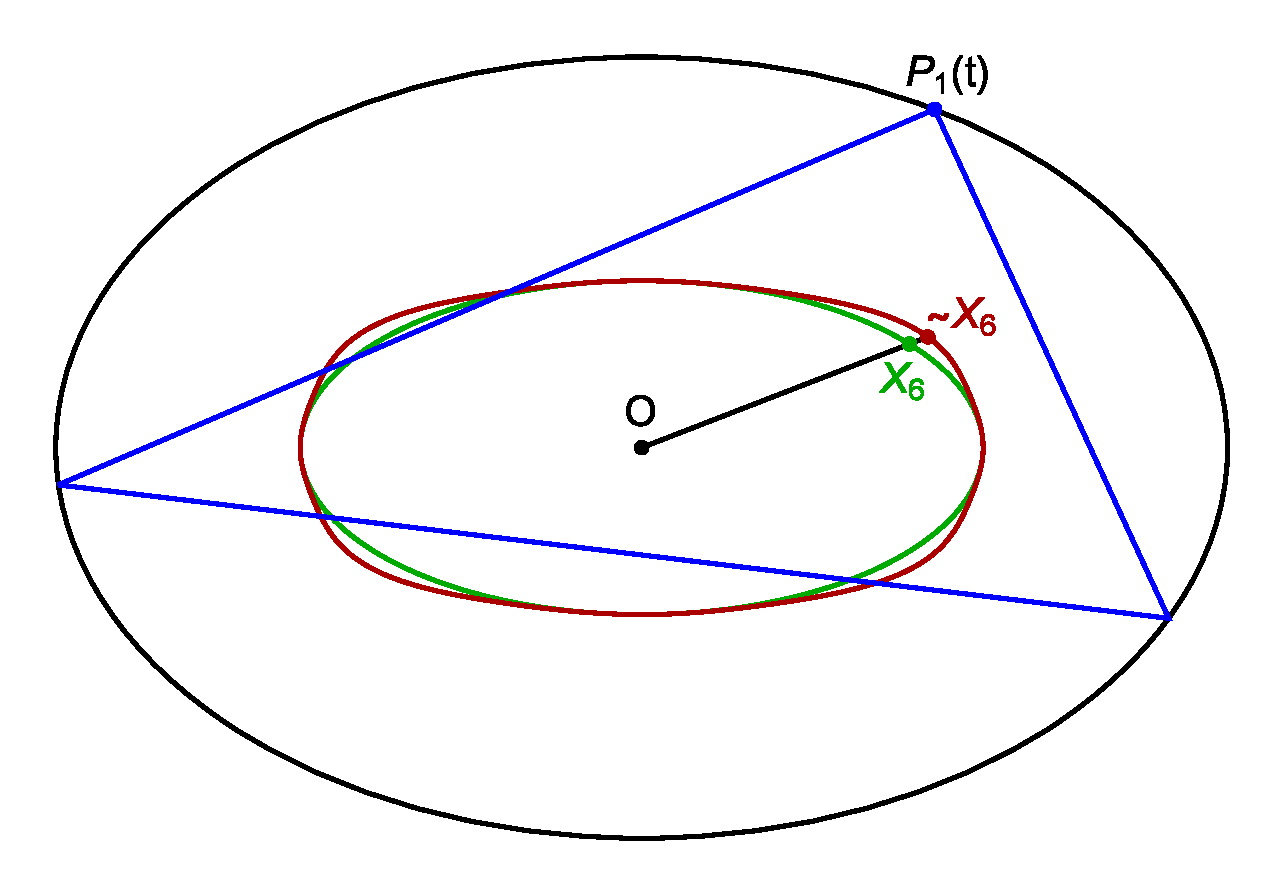
\includegraphics[width=.6\textwidth]{pics_1110_symmedian.eps}
    \caption{An $a/b=1.5$ EB is shown (black) as well as a sample 3-periodic (blue). At this aspect ratio, the locus of $X_6$ (green) is indistinguishable to the naked eye from a perfect ellipse. To see it is non-elliptic, consider the locus of a point ${\sim}X_6(t)=X_6(t)+k|X_6(t)-Y_6'(t)|$, with $k=2{\times}10^6$ and $Y_6'(t)$ the intersection of $OX_6(t)$ with a best-fit ellipse (visually indistinguishable from green), \eqref{eqn:x6-ellipse}. \href{https://bit.ly/3qc0Z0L}{app}}
    \label{fig:symmedian}
\end{figure}

Table~\ref{tab:quartic-coeffs} shows the above coefficients numerically for a few values of $a/b$.

\begin{table}[H]
    \centering
$$
\begin{array}{|c|c|c|c|c|c|c|c|}
\hline
 \text{a/b} & a_6 & b_6 & c_1/c_3 & c_2/c_3 & c_4/c_3 & c_5/c_3 & A(\mathcal{E}_6)/A(\mathcal{X}_6) \\
 \hline
  1.25 & 0.433 & 0.282 & 0.211 & 1.185 & -0.040 & -0.095 & 0.9999 \\
 1.50 & 0.874 & 0.427 & 0.114 & 2.184 & -0.087 & -0.399 & 0.9998 \\
 2.00 & 1.612 & 0.549 & 0.052 & 4.850 & -0.134 & -1.461 & 0.9983 \\
 3.00 & 2.791 & 0.620 & 0.020 & 12.423 & -0.157 & -4.769 & 0.9949 \\
 \hline
\end{array}
$$
\caption{Coefficients $c_i/c_3$, $i=1,2,4,5$ for the quartic locus of $X_6$ as well as the axes $a_6,b_6$ for the best-fit ellipse, for various values of $a/b$. The last-column reports the area ratio of the internal ellipse $\mathcal{E}_6$ (with axes $a_6,b_6$) to that of the quartic locus $\mathcal{X}_6$, showing an almost exact match.}
\label{tab:quartic-coeffs}
\end{table}

\subsection{Locus Triple Winding}
\label{sec:triple-winding}

As an illustration of Lemma~\ref{lem:center-cover}, consider the elliptic locus of $X_1$, the Incenter\footnote{The same argument is valid for the non-elliptic locus of, e.g., $X_{59}$, Figure~\ref{fig:incenter-loci} (right).}. Consider the locus of a point $Y_1$ located on between $X_1$ and an Intouchpoint $I_1$, Figure~\ref{fig:incenter-loci} (left):
 
\begin{equation*}
Y_1(t;\rho)=(1-{\rho})X_1(t)+{\rho}I_1(t),\;\;\;\rho\in[0,1]
 \end{equation*}
 
\noindent When $\rho=1$ (resp. $0$), $Y_1(t)$ is the two-lobe locus of the Intouchpoints (resp. the elliptic locus of $X_1$). With $\rho$ just above zero, $Y_1$ winds thrice around the EB center. At $\rho=0$, the two lobes and the remainder of the locus become one and the same: $Y_1$ winds thrice over the locus of the Incenter, i.e., the latter is the limit of such a convex combination.

It can be shown that at $\rho=\rho^*$, with $\rho^*=1-(b/a)^2$, the two $Y_1(t)$ lobes touch at the the EB center. When $\rho>\rho^*$ (resp. $\rho<\rho^*$), the locus of $Y_1(t)$ has winding number 1 (resp. 3) with respect to the EB center, see Figure~\ref{fig:inc-wind3}.

A similar phenomenon occurs for loci of convex combinations of the following pairs: (i) Barycenter $X_2$ and a side midpoint, (ii) Circumcenter $X_3$ and a side midpoint, (iii) Orthocenter $X_4$ and altitude foot, etc., see \cite[pl\#11,12]{dsr_playlist_2020}.

\begin{figure}
    \centering
    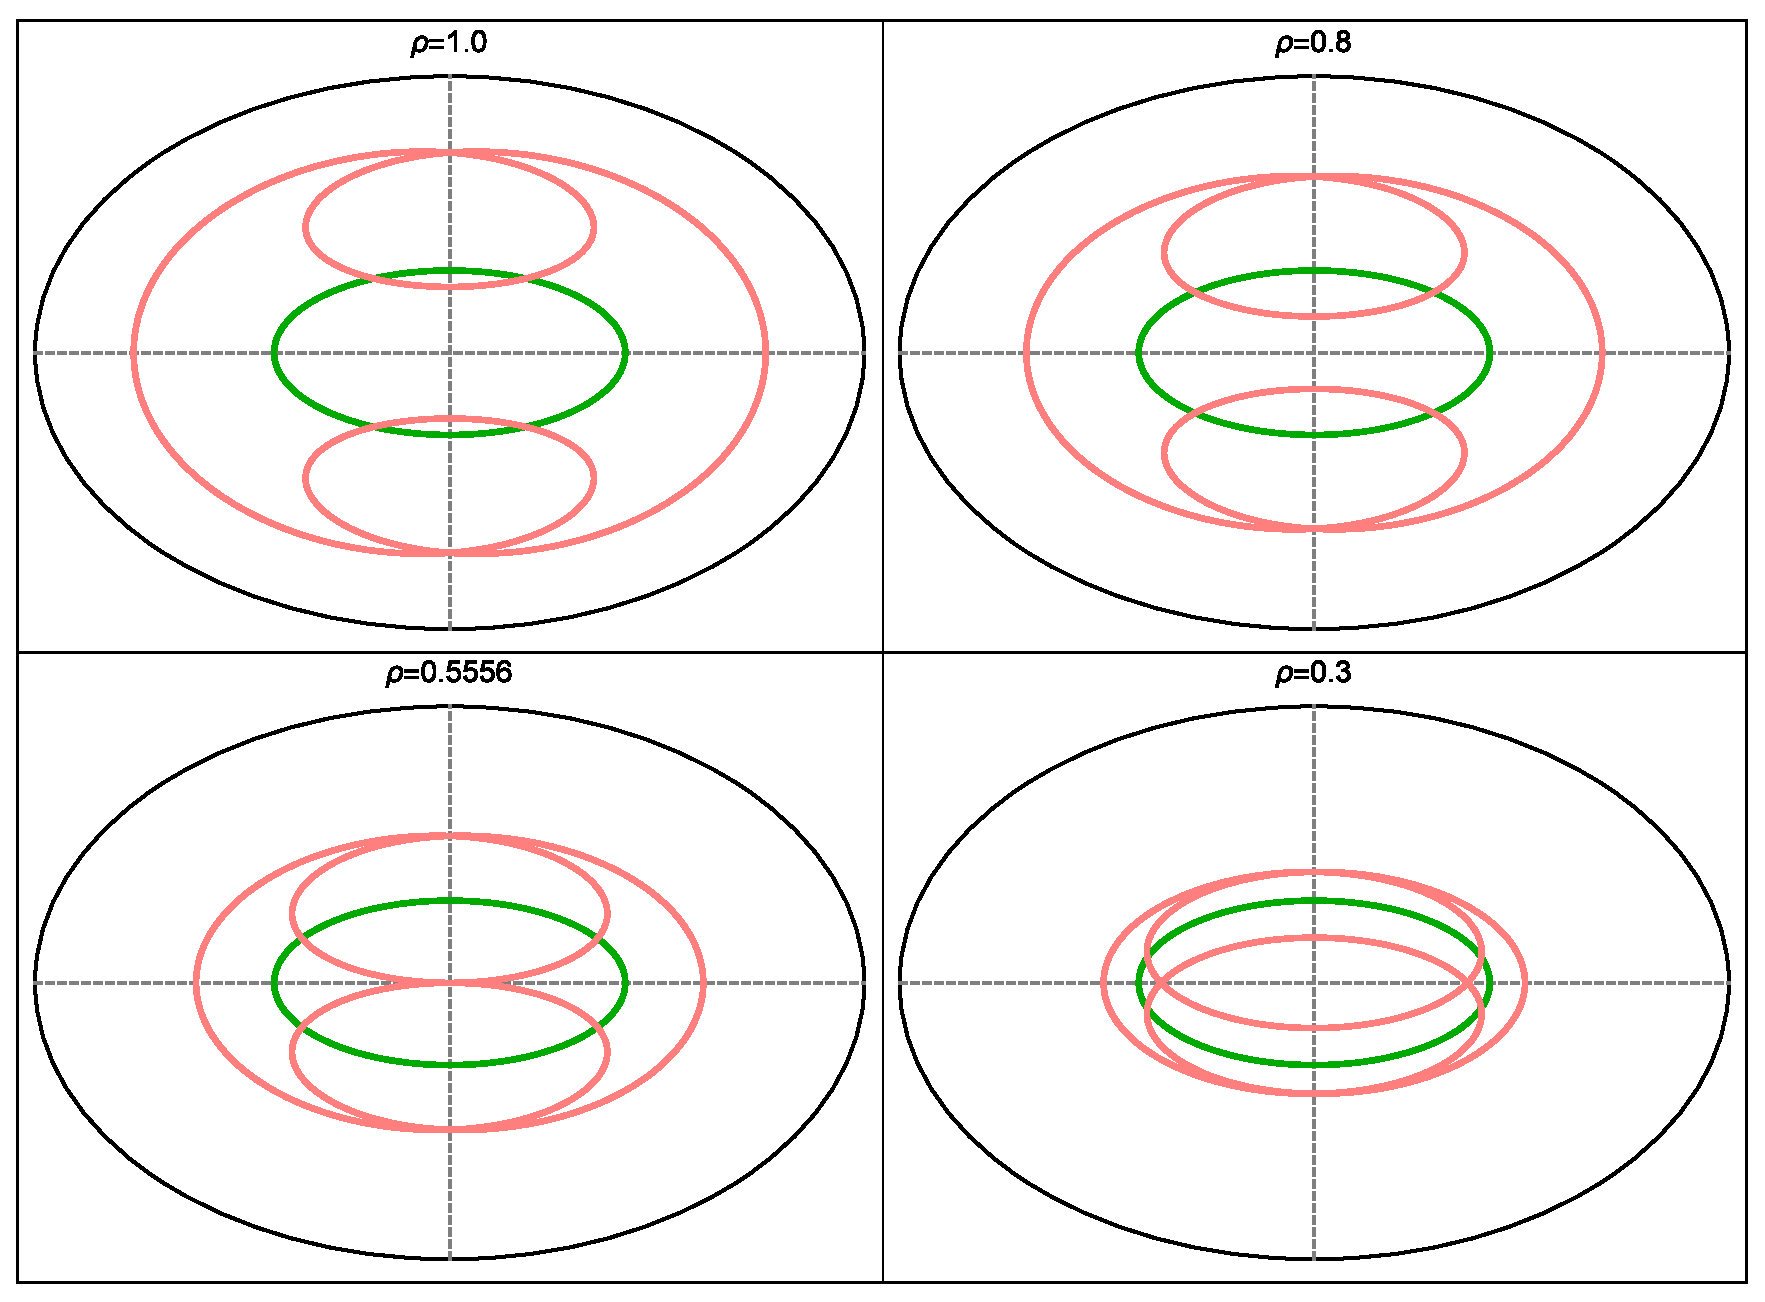
\includegraphics[width=\textwidth]{pics_1090_conv_inc_pedal.eps}
    \caption{An $a/b=1.5$ EB is shown (black) as well as the elliptic locus of $X_1$ (green) and the locus of $Y_1(t)$ (pink), the convex combination of $X_1(t)$ and an Intouchpoint given by a parameter $\rho\in[0,1]$, see Figure~\ref{fig:incenter-loci}(left). At $\rho=1$ (top-left), $Y_1(t)$ is the two-lobe locus of the Intouchpoint. For every tour of an orbit vertex $P_1(t)$ around the EB, $Y_1(t)$ winds once over its locus. At $\rho=0.8$ (top-right) the lobes approach each other but still lie in different half planes. At $\rho=\rho^*=1-(b/a)^2$, the lobes touch at the EB center (bottom-left). If $\rho\in(0,\rho^*)$, the two lobes self-intersect twice. As $\rho{\rightarrow}0$, the two lobes become nearly coincidental (bottom-right). At $\rho=0$, the $Y_1$ locus with its two lobes all collapse to the Incenter locus ellipse (green), in such a way that for every tour of $P_1(t)$ around the EB, $X_1$ winds thrice over its locus. \href{https://youtu.be/3Gr3Nh5-jHs}{Video 1}, \href{https://youtu.be/HZFjkWD_CnE}{Video 2}}
    \label{fig:inc-wind3}
\end{figure}
 

\section{Toward a Typification of Loci}
\label{sec:algebraic}
Our use of a few dozen centers listed in \cite{etc} was a means to validate our approach. In general we would like to predict locus type based on any triangle function, hand-curated or not. Below we take a few steps toward building a practical Computational Algebraic Geometry context useful for practitioners.

\subsection{Trilinears: No Apparent Pattern}

When one looks at a few examples of Triangle Centers whose loci are elliptic vs non, one finds no apparent algebraic pattern in said Trilinears, Table~\ref{tab:center-trilinears}. 

\begin{table}[H]
\scriptsize
\begin{tabular}{|c|l|l|}
\hline
center & name & $h(s_1,s_2,s_3)$ \\
\hline
$X_{1}$ & Incenter & $1$ \\
$X_{2}$ & Centroid & $1/s_1$  \\
$X_{3}$ & Circumcenter & $s_1(s_2^2+s_3^2-s_1^2)$  \\
$X_{4}$ & Orthocenter & $1/[s_1(s_2^2+s_3^2-s_1^2)]$ \\
$X_{5}$ & 9-Point Center & ${s_2}{s_3}[s_1^2(s_2^2+s_3^2)-(s_2^2-s_3^2)^2]$ \\
$X_{11}$ & Feuerbach Point &  ${s_2}{s_3}(s_2+s_3-s_1)(s_2-s_3)^2$ \\
$X_{88}$ & Isog. Conjug. of $X_{44}$ & $1/(s_2+s_3-2{s_1})$ \\
$X_{100}$ & Anticomplement of $X_{11}$ & $1/(s_2-s_3)$  \\ 
\hline
$\mathbf{X_{6}}$ & \textbf{Symmedian Point} & $\mathbf{s_1}$  \\
$\mathbf{X_{13}^*}$ & \textbf{Fermat Point} & $\mathbf{s_1^4 - 2(s_2^2 - s_3^2)^2 + s_1^2(s_2^2 + s_3^2 + 4\sqrt{3}A)}$ \\
$\mathbf{X_{15}^*}$ & \textbf{2nd Isodynamic Point} & $\mathbf{s_1[\sqrt{3}(s_1^2 - s_2^2 - s_3^2) - 4 A]}$ \\
$\mathbf{X_{19}}$ & \textbf{Clawson Point} & $\mathbf{1/(s_2^2 + s_3^2 - s_1^2)}$ \\ 
$\mathbf{X_{37}}$ & \textbf{Crosspoint of $\mathbf{X_{1},X_{2}}$} & $\mathbf{s_2+s_3}$ \\
$\mathbf{X_{59}}$ & \textbf{Isog. Conj. of $\mathbf{X_{11}}$} & $\mathbf{1/[{s_2}{s_3}(s_2+s_3-s_1)(s_2-s_3)^2]}$ \\
\hline
$X_{9}$ & \text{Mittenpunkt} & $s_2+s_3-s_1$ \\
\hline
\end{tabular}
\caption{Triangle Center Function $h$ for a few selected $X_i$'s, taken from \cite{etc}. The first 8 centers produce elliptic loci, whereas the remainder (\textbf{boldfaced}) do not. $X_{13}$ and $X_{15}$ are {\em starred} to indicate their Trilinears are irrational: these contain $A$, the area the triangle, known (e.g., from Heron's formula) to be irrational on the sidelengths. We haven't yet detected an algebraic pattern which differentiates both groups, nor have wre detected an irrational Center whose locus is elliptic. Regarding the last row, the Mittenpunkt, we don't consider its locus to be elliptic since it degenerates to a point at the EB center.}
\label{tab:center-trilinears}
\end{table}

A few observations include:

\begin{itemize}
\item The locus of a Triangle Center is symmetric about both EB axes, Lemma~\ref{lem:axisymmetric}, Section~\ref{sec:algebraic}.
\item There are Trilinears Centers rational on the sidelengths which produce (i) elliptic loci (e.g., $X_1,X_2$, etc.) as well as (ii) non-elliptic (e.g., $X_6$, $X_{19}$, etc.).
\item No locus has been found with more than 6 intersections with a straight line, suggesting the degree is at most 6.
\item No Center has been found with irrational Trilinears whose locus is an ellipse\footnote{Not shown, but also tested were irrational  Triangle Centers $X_j$, $j=14,\,16,\,17,\,18,\,359,\,360,\,364,\,365,\,367$.}, suggesting that the locus of irrational Centers is always non-elliptic.
\end{itemize}

\subsection{An Algebro-Geometric Ambient}

Given EB semi-axes $a,b$, our pro\-blem can be described by the following 14 variables:

\begin{itemize}

\item  6 triangle vertex coordinates, $P_i= (x_i, y_i), \, i=1,2,3$; 

\item 3 sidelengths $s_1, s_2, s_3$;

\item 3 Trilinears  $p,q,r$;
\item  2 locus coordinates $x,y$.
\end{itemize}

These are related by the following system of 14 polynomial equations:

$$
\scriptsize
\begin{array}{|c|l|l|}
\hline
\textbf{eqns.} & \textbf{description} & \textbf{zero set of} \\
\hline
3 & \text{vertices on the EB} & (x_i/a)^2 + (y_i/b)^2 - 1\;,i = 1,2,3 \\
\hline
3 & \begin{array}{l} \text{reflection law at $P_j$} \\ j,k,\ell\;\text{cyclic}, \mathcal{A}=\text{diag}(1/a^2;1/b^2)\end{array} &
\begin{array}{l}
(\mathcal{A} P_j . P_{\ell}- \mathcal{A} P_j.P_j)(P_k-P_j)^2 \\
\;\;\;-(\mathcal{A} P_j . P_k -  \mathcal{A} P_j . P_j) (P_{\ell} - P_j )^2
\end{array} \\
\hline
3 & \text{sidelengths} & (x_i-x_j)^2 + (y_i-y_j)^2 -  s_k^2 \\
\hline
2 & \text{locus Cartesians, \eqref{eqn:trilin-cartesian}} & (p s_1 + q s_2 + r s_3) (x, y) - p s_1 P_1 + q s_2 P_2 + r s_3 P_3 \\
\hline
3 & \text{trilinears (must rationalize)} & p - h(s_1, s_2, s_3);\; q- h(s_2, s_3, s_1);\; r- h(s_3, s_1, s_2) \\
\hline
\end{array}
$$

Billiard Integrability (Appendix~\ref{app:billiards}) implies that out of the first 6 equations, one is functionally dependent on the rest. Therefore, we have 13 independent equations in 14 variables, yielding a 1d algebraic variety, which can be complexified if desired.

Can tools from computational Algebraic Geometry \cite{Schenck2003-GA,Sturmfels97-resultants} be used to eliminate 12 variables automatically, thus obtaining a single polynomial equation $\mathcal{L}(x,y)=0$ whose Zariski closure contains the locus? Below we provide a method based on the theory of resultants \cite{lang,Sturmfels97-resultants} to compute $\mathcal{L}$ for a subset of Triangle Centers.

\subsection{When Trilinears are Rational}
\label{sec:rational-trilinears}

Consider a Triangle Center $X$ whose Trilinears $p:q:r$ are rational on the sidelengths $s_1,s_2,s_3$, i.e., the Triangle Center Function $h$ is rational, equation \eqref{eqn:ftrilins}.

\begin{theorem}
The locus of a rational triangle center is an algebraic curve.
\label{thm:rational-center}
\end{theorem}

Our proof is based on the following 3-steps which yield an algebraic curve $\mathcal{L}(x,y)=0$ which contains the locus. We refer to Lemmas \ref{lem:1coord} and \ref{lem:2sides} appearing below. Appendix~\ref{app:rational-support} contains  supporting expressions.

\begin{proof}

\begin{step}
Introduce the symbolic variables $u, u_1, u_2$:

\begin{equation*}
    u^2 + u_1^2 = 1,\;\;\;\rho_1\, u^2 + u_2^2 = 1.
\end{equation*} % \smallskip

\end{step}
 
\noindent The vertices will be given by rational functions of   $u, u_1, u_2$ 
\begin{equation*} P_1 = (a\,u, b\,u_1),\;\;P_2 = (p_{2x}, p_{2y})/q_2,\;\;\;P_3 = (p_{3x}, p_{3y})/q_3 
\end{equation*}
 
\noindent Expressions for $P_1,P_2,P_3$ appear in Appendix \ref{app:rational-support} as do equations $g_i=0$, $i=1,2,3$, polynomial in $ s_i,u,u_1,u_2$.
 
\begin{step}Express the locus  $X$ as a  rational function on  $u,u_1, u_2, s_1, s_2, s_3$.
\end{step}

Convert $p:q:r$ to Cartesians $ X = (x,y)$ via Equation~\eqref{eqn:trilin-cartesian}. From Lemma~\ref{lem:1coord}, it follows that
$\left(x,y\right)$ is rational on $u,u_1,u_2,s_1,s_2,s_3$.

\begin{equation*} x=\mathcal{Q}/\mathcal{R},\;\;\;y=\mathcal{S}/\mathcal{T}
\end{equation*}

\noindent To obtain the polynomials    $\mathcal{Q,R,S,T}$  on said variables $u,u_1,u_2,s_1,s_2,s_3$,
 one substitutes the 
$p,q,r$ by the corresponding rational functions of  $s_1, s_2, s_3$ that define a specific Triangle Center $X$. Other than that, the method proceeds identically.

\begin{step}
Computing resultants.
Our problem is now cast in terms of the polynomial equations:

\begin{equation*}
E_0= \mathcal{Q}-x\,\mathcal{R}=0,\;\;\; F_0= \mathcal{S}-y\,\mathcal{T}=0
\end{equation*}

\end{step}

%Let $g_1$, $g_2$ and $g_3$ be the polynomials in Appendix~\ref{app:alg_locus}. 
Firstly, compute the resultants, in chain fashion:  

\begin{align*}
    E_1=&\textrm{Res}(g_1,E_0,s_1)=0,\;\;\;F_1=\textrm{Res}(g_1,F_0,s_1)=0\\
	E_2=&\textrm{Res}(g_2,E_1,s_2)=0,\;\;\;F_2=\textrm{Res}(g_2,F_1,s_2)=0\\
	E_3=&\textrm{Res}(g_3,E_2,s_3)=0,\;\;\;F_3=\;\textrm{Res}(g_3,F_2,s_3)=0
\end{align*}
		 
It follows that  $E_3(x,u,u_1,u_2)=0$ and $F_3(y,u,u_1,u_2)=0$ are polynomial
equations. In other words, $s_1, s_2, s_3$ have been eliminated. 

Now  eliminate the variables $u_1$ and $u_2$ by taking the following resultants:

\begin{align*}
	E_4(x,u,u_2)=&\textrm{Res}(E_3,u_1^2+u^2-1,u_1)=0\\ 	F_4(y,u,u_2)=&\textrm{Res}(F_3,u_1^2+u^2-1,u_1)=0\\
	E_5(x,u)=&\textrm{Res}(E_4,u_2^2+\rho_1 u^2-1,u_2)=0\\
	F_5(y,u)=&\textrm{Res}(F_4,u_2^2+\rho_1 u^2-1,u_2)=0
\end{align*}

This yields two polynomial equations $E_5(x,u)=0$ and $F_5(y,u)=0$. 

Finally compute the resultant
$$ {\mathcal L} = \textrm{Res}(E_5,F_5,u)=0
$$
that eliminates $u$ and gives  the implicit algebraic equation for the locus $X$. 
\end{proof}

\begin{remark}
In practice,  after  obtaining  a resultant, a human assists the CAS by factoring out spurious branches
(when recognized), in order to get the final answer in more reduced form.   
\end{remark}

When not rational in the sidelengths, except a few cases\footnote{For instance Hofstadter points $X(359), X(360)$.}, Triangle Centers
in Kimberling's list have explicit Trilinears involving fractional powers and/or terms containing the triangle area. Those can be made implicit, i.e,
given by zero sets of polynomials involving $p,q,r, s_1, s_2, s_3$.  The chain of resultants to be computed will be increased by three, in order to eliminate the variables $p,q, r$ before (or after) $s_1, s_2, s_3$.

\subsubsection{Supporting Lemmas}
\label{sec:supporting-lemmas}

\begin{lemma}
\label{lem:1coord}
Let $P_1=({a}{u},b\sqrt{1-u^2}).$
	The coordinates of $P_2$ and $P_3$ of the 3-periodic billiard orbit are rational functions in the variables $u, u_1, u_2$, where
	$u_1=\sqrt{1-u^2}$, $u_2=\sqrt{1-\rho_1 u^2}$ 
	% and %$u_3=\sqrt{1-\rho_2u^2}$,
and
	$\rho_1=c^4(b^2+\delta)^2/a^6$. % and $\rho_2= (a^2-b^2)/a^2$.
		
	\end{lemma}
	
	\begin{proof}
	Follows directly from the parametrization of the billiard orbit, Appendix~\ref{app:p1p2p3}. In fact,  $P_2=(x_2(u),y_2(u)) =( p_{2x}/q_2, p_{2y}/q_2)$ and $P_3=(x_3(u),y_3(u))$ $=( p_{3x}/q_3, p_{3y}/q_3)$, where $p_{2x}$, $p_{2y}$, $p_{3x}$ and $p_{3y}$ have degree $4$ in $(u,u_1,u_2)$  and $q_2$, $q_3$ are algebraic of degree $4$ in $u$. Expressions for $u_1,u_2$ appear in Appendix~\ref{app:exit-angle}.
\end{proof}
	
\begin{lemma}
\label{lem:2sides} Let $P_1=(a u,b\sqrt{1-u^2}).$ Let $s_1$, $s_2$ and $s_3$ the sides of the triangular orbit ${P_1}{P_2}{P_3}$. Then $g_1(u,s_1)=0$, $g_2(s_2,u_2,u)=0$ and $g_3(s_3,u_2,u)=0$ for polynomial functions $g_i$.  
\end{lemma}
	
\begin{proof}
Using the parametrization of the 3-periodic billiard orbit it follows that $s_1^2-|P_2-P_3|^2=0$ is a rational equation in the variables $u,s_1$. Simplifying, leads to $g_1(s_1,u)=0.$

Analogously for $s_2$ and $s_3$. In this case, the equations $s_2^2-|P_1-P_3|^2=0$ and  $s_3^2-|P_1-P_2|^2=0$   have   square roots $u_2=\sqrt{1-\rho_1 u^2}$ and $u_1=\sqrt{1-u^2}$ and  are rational in the variables $s_2,u_2,u_1,u$ and $s_3,u_2,u_1,u$ respectively. It follows that the degrees of $g_1$, $g_2$, and $g_3$ are $10$.  Simplifying, leads to $g_2(s_2,u_2,u_1,u)=0 $ and $g_3(s_3,u_2,u_1,u)=0$. 
\end{proof}

\subsection{Examples}

Table~\ref{tab:zariski} shows the Zariski closure obtained contained the elliptic locus of a few Triangle Centers. Notice one factor is always of the form $[(x/a_i)^2+(y/b_i)^2)-1]^3$, related to the triple cover described in Section~\ref{sec:triple-winding}. The expressions shown required some manual simplification during the symbolic calculations. 

\begin{table}
$$
\scriptsize
\begin{array}{|c|l|l|l|l|l|}
\hline
X_i & \text{Name} & \text{Spurious Factors} & \text{Elliptic Factor} & a_i & b_i \\
\hline
1 & \text{Incenter} & \text{very long expression} & \begin{array}{l}
[36 (91 + 61 \sqrt{61}) x^2 \\
+ 324 (139 + 19 \sqrt{61}) y^2 \\
+ 22761 - 3969 \sqrt{61}]^6
\end{array} & 0.63504 & 0.29744 \\
\hline
2 & \text{Barycenter} & \begin{array}{l} (91500x^2\\
+49922\sqrt{61}-370993)^2 \end{array} & \begin{array}{l} (100x^2\\+225y^2\\
+52\sqrt{61}-413)^3 \end{array} & 0.26205 & 0.1747 \\
\hline
3 & \text{Circumcenter} & \begin{array}{l}
x\\(3600 x^4-6380 x^2-1539)\\
(40 x^2+5\sqrt{61}-43)^2\\
\begin{array}{l}
(-1104500 y^2\\+591136\sqrt{61}-4633685)^2\end{array}\\
(65880x^2+8527\sqrt{61}-64649)^6 \end{array} & \begin{array}{l}
(5832 x^2\\
+(2752-320\sqrt{61}) y^2\\5751-729\sqrt{61})^3 \end{array} & 0.099146 & 0.4763\\
\hline
\end{array}
$$
\caption{Method of Resultants applied to obtain the Zariski closure for a few sample Triangle Centers with elliptic loci, for the specific case of $a/b=1.5$. Both spurious and an elliptic factor are present. The latter are raised to powers multiple of three suggesting a phenomenon related to the triple cover, Section~\ref{sec:triple-winding}. Also shown are semi-axes $a_i,b_i$ implied by the elliptic factor. These have been checked to be in perfect agreement with the values predicted for those semi-axes in \cite{garcia2019-incenter}.}
\label{tab:zariski}
\end{table}



\section{Conclusion}
\label{sec:conclusion}
A few interesting questions are posed to the reader.

\begin{itemize}
    \item Are there conditions in the Trilinears of a Triangle Center so that its locus is an ellipse? Please refer to
    Table~\ref{tab:center-trilinears} for a few examples showing no apparent pattern.
    \item Can the degree of the locus of a Triangle Center or Derived Triangle vertex be predicted based on its Trilinears?
    \item Is there a Triangle Center such that its locus intersects a straight line more than 6 times?
    \item Certain Triangles Centers have non-convex loci (e.g., $X_{67}$ at $a/b=1.5$ \cite{dsr_locus_gallery_2019}). What determines non-convexity?
    \item What determines the number of self-intersections of a given locus?
    \item In the spirit of \cite{corentin19,olga14}, how would one determine via complex analytic geometry, that $X_6$ is a quartic?
    \item What is the non-elliptic locus described by the summits of equilaterals erected over each orbit side (used in the construction of the Outer Napoleon Triangle \cite{mw}).  \cite[pl\#13]{dsr_playlist_2020}. What kind of curve is it?
    \item Within $X_1$ and $X_{100}$ only $X_i$, $i=13{\ldots}18$ have irrational Trilinears. $X_j$, $j=359,\,360,\,364,\,365,\,367$ are irrational and have loci which numerically are non-elliptic. Can any irrational Center produce an ellipse?
    \item $X_6$ is the isogonal conjugate of $X_2$. Though the latter's locus is an ellipse, the former's is a quartic. In the case of the isogonal pair $X_3$ and $X_4$ both are ellipses. What is the connection with isogonal (and/or isotomic transformations) and ellipticity?
\end{itemize}

\subsection{Videos and Media}

The reader is encouraged to browse our companion paper \cite{reznik2020-ballet} where intriguing locus phenomena are investigated. Additionally, loci can be explored interactively with our browser-based  \href{https://dan-reznik.github.io/ellipse-mounted-loci-p5js/}{app} \cite{darlan2020-ellipse-mounted}.

Videos mentioned herein are on a \href{https://bit.ly/2REOigc}{playlist} \cite{dsr_playlist_2020}, with links provided on Table~\ref{tab:playlist}.

\begin{table}
\small
\begin{tabular}{|c|l|l|l|}
\hline
{id} & Title & Section & \texttt{youtu.be/<.>}\\
\hline
{01} &
{Locus of $X_1$ is an Ellipse} & \ref{sec:intro} & \href{https://youtu.be/BBsyM7RnswA}{\texttt{BsyM7RnswA}} \\
{02} &
{Locus of Intouchpoints is non-elliptic} & \ref{sec:intro}, \ref{app:early} & \href{https://youtu.be/9xU6T7hQMzs}{\texttt{9xU6T7hQMzs}}\\
{03} &
{$X_9$ stationary at EB center} & \ref{sec:intro} & \href{https://youtu.be/tMrBqfRBYik}{\texttt{tMrBqfRBYik}} \\
{04} &
{Stationary Excentral Cosine Circle}  &
\ref{sec:intro} & \href{https://youtu.be/ACinCf-D_Ok}{\texttt{ACinCf-D\_Ok}} \\
{05} &
{Loci for $X_1\ldots{X_5}$ are ellipses} &
\ref{app:early} & \href{https://youtu.be/sMcNzcYaqtg}{\texttt{sMcNzcYaqtg}} \\
{06} &
{Elliptic locus of Excenters similar to rotated $X_1$} &
\ref{app:early} & \href{https://youtu.be/Xxr1DUo19_w}{\texttt{Xxr1DUo19\_w}} \\
{07} &
{Loci of $X_{11}$, $X_{100}$ and Extouchpoints are the EB} &\ref{app:early} & \href{https://youtu.be/TXdg7tUl8lc}{\texttt{TXdg7tUl8lc}} \\
{08} &
{Family of Derived Triangles} &
\ref{sec:loci_geom} & \href{https://youtu.be/xyroRTEVNDc}{\texttt{xyroRTEVNDc}} \\
{09} &
{Loci of Vertices of Derived Triangles} &
 \ref{app:early},\ref{sec:loci_geom}& \href{https://youtu.be/OGvCQbYqJyI}{\texttt{OGvCQbYqJyI}} \\
{10} &
{Peter Moses' 29 Billiard Points} &
\ref{sec:loci_geom} & \href{https://youtu.be/JdcJt5PExsw}{\texttt{JdcJt5PExsw}}\\
{11} &
{Convex Comb.: $X_1$-Intouch and $X_2$-Midpoint} &
\ref{sec:triple-winding} & \href{https://youtu.be/3Gr3Nh5-jHs}{\texttt{3Gr3Nh5-jHs}}\\
{12} &
{Convex Comb.: $X_3$-Midpoint and $X_4$-Altfoot} &
\ref{sec:triple-winding} & \href{https://youtu.be/HZFjkWD_CnE}{\texttt{HZFjkWD\_CnE}}\\
{13} &
{Oval Locus of the Outer Napoleon Summits} &
\ref{sec:conclusion} & \href{https://youtu.be/70-E-NZrNCQ}{\texttt{70-E-NZrNCQ}} \\
\hline
\end{tabular}
\caption{Videos mentioned in the paper available in a Youtube playlist \cite{dsr_playlist_2020}. The last column contains a clickable YouTube code.}
\label{tab:playlist}
\end{table}



\section*{Acknowledgments}
We warmly thank Clark Kimberling, Peter Moses, Sergei Tabachnikov, Richard Schwartz, Arseniy Akopyan, Olga Romaskevich, Ethan Cotterill, for their invaluable input during this research.

The first author is fellow of CNPq and coordinator of Project PRONEX/ CNPq/ FAPEG 2017 10 26 7000 508.

%\begin{thebibliography}{10}
\providecommand{\url}[1]{{#1}}
\providecommand{\urlprefix}{URL }
\expandafter\ifx\csname urlstyle\endcsname\relax
  \providecommand{\doi}[1]{DOI~\discretionary{}{}{}#1}\else
  \providecommand{\doi}{DOI~\discretionary{}{}{}\begingroup
  \urlstyle{rm}\Url}\fi

\bibitem{akopyan2020-invariants}
Akopyan, A., Schwartz, R., Tabachnikov, S.: Billiards in ellipses revisited
  (2020).
\newblock \urlprefix\url{https://arxiv.org/abs/2001.02934}.
\newblock Ar{X}iv

\bibitem{bialy2020-invariants}
Bialy, M., Tabachnikov, S.: {Dan Reznik's} identities and more (2020).
\newblock \urlprefix\url{https://arxiv.org/abs/2001.08469}.
\newblock Ar{X}iv

\bibitem{cox2005-AG}
Cox, D., Little, J., O'Shea, D.: Using Algebraic Geometry.
\newblock Springer (2005)

\bibitem{dragovic11}
Dragovi\'{c}, V., Radnovi\'{c}, M.: Poncelet Porisms and Beyond: Integrable
  Billiards, Hyperelliptic Jacobians and Pencils of Quadrics.
\newblock Frontiers in Mathematics. Springer, Basel (2011).
\newblock \urlprefix\url{https://books.google.com.br/books?id=QcOmDAEACAAJ}

\bibitem{corentin19}
Fierobe, C.: On the circumcenters of triangular orbits in elliptic billiard
  (2018).
\newblock \urlprefix\url{https://arxiv.org/pdf/1807.11903.pdf}.
\newblock Submitted %to {l'Enseign. Math.}

\bibitem{fitzgibbon99-ellipse}
Fitzgibbon, A., Pilu, M., Fisher, R.: Direct least square fitting of ellipses.
\newblock Pattern Analysis and Machine Intelligence \textbf{21}(5) (1999)

\bibitem{ronaldo19}
Garcia, R.: Elliptic billiards and ellipses associated to the 3-periodic
  orbits.
\newblock American Mathematical Monthly \textbf{126}(06), 491--504 (2019).
\newblock \urlprefix\url{https://doi.org/10.1080/00029890.2019.1593087}

\bibitem{griffiths1978}
Griffiths, P., Harris, J.: On {C}ayley's explicit solution to {P}oncelet's
  porism.
\newblock Enseign. Math. (2) \textbf{24}(1-2), 31--40 (1978)

\bibitem{dekov14}
Grozdev, S., Dekov, D.: The computer program “discoverer” as a tool of
  mathematical investigation.
\newblock International Journal of Computer Discovered Mathematics (IJCDM)
  (2014).
\newblock \urlprefix\url{http://www.ddekov.eu/j/2014/JCGM201405.pdf}

\bibitem{kaloshin2018}
Kaloshin, V., Sorrentino, A.: On the integrability of {B}irkhoff billiards.
\newblock Phil. Trans. R. Soc. \textbf{A}(376) (2018).
\newblock \doi{https://doi.org/10.1098/rsta.2017.0419}

\bibitem{kimberling1993_rocky}
Kimberling, C.: Triangle centers as functions.
\newblock Rocky Mountain J. Math. \textbf{23}(4), 1269--1286 (1993).
\newblock \doi{10.1216/rmjm/1181072493}.
\newblock \urlprefix\url{https://doi.org/10.1216/rmjm/1181072493}

\bibitem{etc}
Kimberling, C.: Encyclopedia of triangle centers (2019).
\newblock
  \urlprefix\url{https://faculty.evansville.edu/ck6/encyclopedia/ETC.html}

\bibitem{lang}
Lang, S.: Algebra, \emph{Graduate Texts in Mathematics}, vol. 211, third edn.
\newblock Springer-Verlag, New York (2002).
\newblock \doi{10.1007/978-1-4613-0041-0}.
\newblock \urlprefix\url{https://doi.org/10.1007/978-1-4613-0041-0}

\bibitem{sergei07_grid}
Levi, M., Tabachnikov, S.: The {P}oncelet grid and billiards in ellipses.
\newblock The American Mathematical Monthly \textbf{114}(10), 895--908 (2007).
\newblock \doi{10.1080/00029890.2007.11920482}.
\newblock \urlprefix\url{https://doi.org/10.1080/00029890.2007.11920482}

\bibitem{moore2009-interval-analysis}
Moore, R., Kearfott, R.B., Cloud, M.J.: Introduction to Interval Analysis.
\newblock SIAM (2009)

\bibitem{dsr_applet_x12345}
Reznik, D.: Applet showing the locus of several triangular centers (2019).
\newblock \urlprefix\url{https://editor.p5js.org/dreznik/full/i1Lin7lt7}

\bibitem{dsr_locus_gallery_2019}
Reznik, D.: Triangular orbits in elliptic billards: Loci of points
  {X(1)~X(100)} (2019).
\newblock
  \urlprefix\url{https://dan-reznik.github.io/Elliptical-Billiards-Triangular-Orbits/loci_6tri.html}

\bibitem{dsr_playlist_2020}
Reznik, D.: Playlist for {``Loci of Triangular Orbits in an Elliptic Billiard:
  Elliptic? Algebraic?''} (2020).
\newblock \urlprefix\url{https://bit.ly/2REOigc}

\bibitem{reznik19}
Reznik, D., Garcia, R., Koiller, J.: Can the elliptic billiard still surprise
  us?
\newblock Mathematical Intelligencer  (2019).
\newblock \doi{10.1007/s00283-019-09951-2}.
\newblock \urlprefix\url{https://arxiv.org/pdf/1911.01515.pdf}

\bibitem{reznik2020-loci}
Reznik, D., Garcia, R., Koiller, J.: Intriguing loci of triangular orbits in
  elliptic billiards (2020).
\newblock In preparation

\bibitem{olga14}
Romaskevich, O.: On the incenters of triangular orbits on elliptic billiards.
\newblock Enseign. Math. \textbf{60}(3-4), 247--255 (2014).
\newblock \doi{10.4171/LEM/60-3/4-2}.
\newblock \urlprefix\url{https://arxiv.org/pdf/1304.7588.pdf}

\bibitem{rozikov2018}
Rozikov, U.A.: An Introduction To Mathematical Billiards.
\newblock World Scientific Publishing Company (2018)

\bibitem{Schenck2003-GA}
Schenck, H.: Computational Algebraic Geometry, London Mathematical Society
  Student Text, vol.~58.
\newblock Cambridge University Press (2003)

\bibitem{snyder92-ellipse}
Snyder, J.M.: Interval analysis for computer graphics.
\newblock Computer Graphics \textbf{26}(2), 121--129 (1992)

\bibitem{Sturmfels97-resultants}
Sturmfels, B.: Introduction to resultants, in Applications of Computational
  Algebraic Geometry, vol.~53, pp. 25--40.
\newblock American Mathematical Society (1997).
\newblock Proceedings of Symposia in Applied Mathematics

\bibitem{sergei91}
Tabachnikov, S.: Geometry and Billiards, \emph{Student Mathematical Library},
  vol.~30.
\newblock American Mathematical Society, Providence, RI (2005).
\newblock \doi{10.1090/stml/030}.
\newblock
  \urlprefix\url{http://www.personal.psu.edu/sot2/books/billiardsgeometry.pdf}.
\newblock Mathematics Advanced Study Semesters, University Park, PA

\bibitem{sergei2016proj}
Tabachnikov, S.: Projective configuration theorems: old wine into new
  wineskins.
\newblock In: S.~Dani, A.~Papadopoulos (eds.) Geometry in History, pp.
  401--434. Springer Verlag (2019).
\newblock \urlprefix\url{https://arxiv.org/pdf/1607.04758.pdf}

\bibitem{mw}
Weisstein, E.: Mathworld (2019).
\newblock \urlprefix\url{http://mathworld.wolfram.com}

\end{thebibliography}


\appendix
%\section{Orbit Vertices}
%\label{app:orbit-vertices}
%Let the boundary of the Billiard satisfy Equation~\eqref{eqn:billiard-f}. Assume, without loss of generality, that $a{\geq}b$.

Given a starting vertex $P_1$ and an exit angle $\alpha$ (as above), the orbit $P_1P_2P_3$ will be such that \cite{ronaldo19}:

vertex $P_2$ will be given by $(p_{2x},p_{2y})/q_2$, with

\begin{align*}
%\label{eqn:p2}
p_{2x}=&-{b}^{4} \left(  \left(   a^2+{b}^{2}\right)\cos^{2}\alpha   -{a}^{2}  \right) x_1^{3}-2\,{a}^{4}{b}^{2} \cos \alpha  \,\sin  \alpha  \,  x_1^{2}{y_1}\\
&+{a}^{4} \left(  ({a
}^{2}-3\, {b}^{2}) \cos^{2} \alpha  +{b}^{2}
 \right) {x_1}\,y_1^{2}-2{a}^{6} \,\cos  \alpha  \sin   \alpha  \, y_1^{3} ,
\\
p_{2y}=& 2{b}^{6} \,\cos \alpha\sin \alpha\,   x_1^{3}+{b}^{4}\left(  ({b
 }^{2}-3\, {a}^{2}) \cos^{2} \alpha  +{a}^{2}
  \right) x_1^{2}{y_1}\\
&+  2\,{a}^{2} {b}^{4}\cos \alpha \sin
  \alpha \; {x_1} y_1^{2} -{
a}^{4}  \left(  \left(   a^2+{b}^{2}\right)\cos^{2}  \alpha  -{b}^{2}  \right)  y_1^{3}
\\
q_2=&{b}^{4} \left( a^2-c^2\cos^2\alpha   \right)
x_1^{2}+{a}^{4} \left(  {b}^{2}+c^2\cos^2 \alpha  
 \right) y_1^{2}\\
 & - 2\, {a}^{2}{b}^{2}{c^2}\cos \alpha\sin \alpha \; {x_1}\,{
y_1}.
\end{align*}

and vertex $P_3$ will be given by $(p_{3x},p_{3y})/q_3$, with:

\begin{align*}
p_{3x}=& {b}^{4} \left( {a}^{2}- \left( {b}^{2}+{a}^{2} \right) \right)
 \cos^{2}  \alpha   x_1^{3} +2\,{a}^{4}{b}^{2} \cos  \alpha \sin \alpha\,   x_1^{2}{ y_1}\\
 &+{a}^{4} \left( 
  \cos^{2}  \alpha  \left( {a}^{2}-3\,{b}^{2}
 \right) +{b}^{2} \right) { x_1}\, y_1^{2} +2\, {a}^{6} 
 \cos \alpha\,\sin \alpha\, y_1^{3}
\\
p_{3y}=& -2\, {b}^{6} \cos \alpha\sin \alpha\, x_1^{3}+{b}^{4} \left( {a}^{2}+ \left( {b}^{2}-3\,{a}^{2} \right)    \cos^2\alpha \right) {{ x_1}}^{2}{ y_1}
\\
& -2\,{a}^{2}  {b}^{4}\cos
 \alpha  \sin \alpha\,  x_1 y_1^{2}+
 {a}^{4} \left( {b}^{2}- \left( {b}^{2}+{a}^{2} \right)   \cos^{2}  \alpha  \right)\,  y_1^{3},
\\
q_3=& {b}^{4} \left( {a}^{2}-{c^2}\cos^{2}\alpha   \right) x_1^{2}+{a}^{4} \left( {b}^{2}+c^2\cos^{2}\alpha  \right)  y_1^{2}\\
&+2\,{a}^{2}{b}^{
2} c^2 \cos\alpha \sin\alpha\, { x_1}\,{ y_1}.
\end{align*}

The sides of the triangular orbit have lengths 
$s_1=\mid P_3-P_2\mid$, $s_2=\mid P_3-P_1\mid$ and
$s_3=\mid P_2-P_1\mid$.

\section{Table of Symbols}
\label{app:symbols}
Tables~\ref{tab:kimberling} and \ref{tab:symbols} lists most Triangle Centers and symbols mentioned in the paper.

\begin{table}
\scriptsize
\begin{tabular}{|c|l|l|}
\hline
Center & Meaning & Note\\
\hline
$X_1$ & Incenter & Locus is Ellipse \\
$X_2$ & Barycenter & Perspector of Steiner Circum/Inellipses \\
$X_3$ & Circumcenter & Locus is Ellipse, Perspector of $M$ \\
$X_4$ & Orthocenter & \makecell[tl]{Exterior to EB\\ when 3-periodic is obtuse} \\
$X_5$ & Center of the 9-Point Circle & \\
$X_6$ & Symmedian Point & Locus is Quartic \cite{garcia2020-ellipses} \\
$X_6^*$ & $X_9$ of Orthic & Detached from $X_6$ locus for obtuse triangles \\
$X_7$ & Gergonne Point & Perspector of Incircle \\
$X_8$ & Nagel Point & Perspector of $I_9$, $X_1$ of ACT Incircle \\
$X_9$ & Mittenpunkt & Center of (Circum)billiard \\
$X_{10}$ & Spieker Point & Incenter of Medial \\
$X_{11}$ & Feuerbach Point & on confocal Caustic \\
$X_{40}$ & Bevan Point & $X_3$ of Excentral \\
$X_{69}$ & $X_6$ of the ACT & Perspector of $I_3$ \\
$X_{100}$ & Anticomplement of $X_{11}$ & On Circumcircle and EB, $J_{exc}$ center \\
$X_{125}$ & Center of Jerabek Hyperbola $J$ & \\
$X_{142}$ & $X_9$ of Medial & Midpoint of $X_9{X_{7}}$, lies on $L(2,7)$ \\ 
$X_{144}$ & Anticomplement of $X_7$ &\makecell[tl]{Perspector of ACT\\and its Intouch Triangle} \\
$X_{168}$ & $X_9$ of the Excentral Triangle &  Non-elliptic Locus\\
$X_{190}$ & Focus of the Yff Parabola & Intersection of $E_2$ and the EB \\
$X_{264}$ & Isotomic Conjugate of $X_3$ & Perspector of $I_5$ \\
$X_{649}$ & Cross-difference of $X_1,X_2$ & Perspector of $J_{exc}$ \\ 
$X_{664}$ &  Trilinear Pole of $L( 2,7)$ & Intersection of $E_1$ and $E_2$ \cite{moses2020-private-circumconic} \\
$X_{650}$ & Cross-difference of $X_1,X_3$ & Perspector of $F$ \\
$X_{1156}$ & \makecell[tl]{Isogonal Conjugate of\\Schröder Point $X_{1155}$} &  intesection of $F$ with EB \\
$X_{1742}$ & Mimosa Transform of $X_{212}$ & Perspector of $I_5'$ \\
$X_{2951}$ & Excentral-Isogonal Conjugate of $X_{57}$ & Perspector of $I_3'$ \\
$X_{3035}$ & Complement of $X_{11}$ & Center of $F_{med}$ \\
$X_{3659}$ & $X_{11}$ of Excentral Triangle & Center of $F_{exc}$ \\
\hline
$L(2,7)$ & ACT-Medial Mittenpunkt Axis & Line $\mathcal{L}_{663}$  \cite{etc_central_lines} \\
$L(1,3)$ & Isogonal Conjugate of $F$ and $J_{exc}$ &  Line $\mathcal{L}_{650}$ \cite{etc_central_lines}  \\
\hline
\end{tabular}
\caption{Kimberling Centers and Central Lines mentioned in paper}
\label{tab:kimberling}
\end{table}

\begin{table}
\scriptsize
\begin{tabular}{|c|l|l|}
\hline
Symbol & Meaning & Note\\
\hline
$a,b$ & EB semi-axes & $a>b>0$\\ 
$P_i,s_i$ & Vertices and sidelengths of 3-periodic & invariant $\sum{s_i}$ \\
$P_i'$ & Vertices of the Excentral Triangle & \\
$a_c,b_c$ & Semi-axes of confocal Caustic & \\ 
$a_9,b_9$ & Semi-axes of Poristic Circumbilliard & \\
$r,R,\rho$ & Inradius, Circumradius, $r/R$ & $\rho$ is invariant \\
$\delta$ & Oft-used constant & $\sqrt{a^4-a^2 b^2+b^4}$ \\
$d$ & Distance $|X_1{X_3}|$ & $\sqrt{R(R-2r)}$\\
%\href{https://youtu.be/DS4ryndDK6Q}{15} & Invariants of the Poristic Triangle Family &
%\ref{sec:conclusion} \\
$\alpha$ & EB aspect ratio & $a/b$ \\
$\alpha_4$ & \makecell[tl]{$a/b$ threshold for obtuse 3-Periodics} & $ \sqrt{2\,\sqrt {2}-1}$\\
$\alpha_{eq}$ & $a/b$ for equilateral Orthic & $\sqrt{4\sqrt{3}-3}$\\
$P^\perp$ & Obtuse 3-periodic limits on EB & \\
$x^*,y^*$ & where $X_6^*$ detaches from $X_6$ locus & Occurs when some $P_i$ is at $P^\perp$\\
\hline
$F,J$ & Feuerbach, Jerabek Hyperbola & Centers $X_{11},X_{125}$, Perspectors $X_{650},X_{647}$ \\
$F_{exc}$ & $F$ of Excentral Triangle & Center $X_{3659}$ \cite{moses2020-private-circumconic} \\
$J_{exc}$ & $J$ of Excentral Triangle & Center $X_{100}$, Perspector $X_{649}$ \\
$F',J_{exc}'$ & $F,J_{exc}$ translated by $-X_{11},-X_{100}$ & Origin-centered \\
$F_{med}$ & $F$ of Medial & Center $X_{3035}$ 
\cite{moses2020-private-circumconic} \\
\hline
$E_i$ & Circumellipse centered on $X_i$ & \makecell[tl]{Axes parallel to $E_9$ if $X_i$ on $F_{med}$} \\
$E_6'$ & Excentral MacBeath Circumellipse & Center $X_9$, Perspector $X_{40}$ \\
\hline
$I_3,I_5$ & Inellipses Centered on $X_3$,$X_5$ & Perspectors $X_{69},X_{264}$ \\
$I_9$ & Mandart Inellipse & Perspector $X_8$ \\
$I'_3$ & Excentral $I_3$ & Center $X_{40}$, Perspector $X_{2951}$ \cite{moses2020-private-circumconic} \\
$I'_5$ & Excentral $I_5$ & Center $X_{3}$, Perspector $X_{1742}$ \cite{moses2020-private-circumconic}\\
\hline
$\eta'_i,\eta_i$ & Major and minor semiaxis of $E_i$ & Invariant ratio if $X_i$ on $F_{med}$\\
$\mu_i',\mu_i$ & Major and minor semiaxis of $I_i'$ & Invariant ratio for $i=3,5$ \\
$\lambda',\lambda$ & Focal lengths of $J_{exc},F$ (and $J_{exc}',F'$) & Invariant ratio \\
\hline
\end{tabular}
\caption{Symbols used in paper}
\label{tab:symbols}
\end{table}

\section{Computing a  Circumconic}
\label{app:circum-linear}
Let a Circumconic have center $M=(x_m,y_m)$ Equation~\eqref{eqn:e0} is subject to the following 5 constraints\footnote{If $M$ is set to $X_9$ one obtains the Circumbilliard.}: it must be satisfied for vertices $P_1,P_2,P_3$, and its gradient must vanish at $M$:

\begin{align*}
f(P_i)=&\;0,\;\;\;i=1,2,3\\
\frac{dg}{dx}(x_m,y_m)=&\;c_1+c_3 y_m+2c_4 x_m=0\\
\frac{dg}{dy}(x_m,y_m)=\;&c_2+c_3 x_m+2c_5 y_m=0
\end{align*}

Written as a linear system:

$$
\left[
\begin{array}{ccccc}
x_1&y_1&x_1 y_1&x_1^2&y_1^2\\
x_2&y_2&x_2 y_2&x_2^2&y_2^2\\
x_3&y_3&x_3 y_3&x_3^2&y_3^2\\
1&0&y_m&2\,x_m&0\\
0&1&x_m&0&2\,y_m
\end{array}
\right] .
\left[\begin{array}{c}c_1\\c_2\\c_3\\c_4\\c_5\end{array}\right] =
\left[\begin{array}{c}-1\\-1\\-1\\0\\0\end{array}\right]
$$

Given sidelenghts $s_1,s_2,s_3$, the coordinates of $X_9=(x_m,y_m)$ can be obtained by converting its Trilinears $\left(s_2 + s_3 - s_1 :: ...\right)$ to Cartesians \cite{etc}. 

Principal axes' directions are given by the eigenvectors of the Hessian matrix $H$ (the jacobian of the gradient), whose entries only depend on $c_3$, $c_4$, and $c_5$:

\begin{equation}
H = J(\nabla{g})=\left[\begin{array}{cc}2\,c_4&c_3\\c_3&2\,c_5\end{array}\right]
\label{eqn:hessian}
\end{equation}

The ratio of semiaxes' lengths is given by the square root of the ratio of $H$'s eigenvalues:

\begin{equation}
a/b=\sqrt{\lambda_2/\lambda_1}
\label{eqn:ratiolambda}
\end{equation}

Let $U=(x_u,y_u)$ be an eigenvector of $H$. The length of the semiaxis along $u$ is given by the distance $t$ which satisfies:

$$
g(M + t\,U) = 0
$$

This yields a two-parameter quadratic $d_0 + d_2 t^2$, where:

$$
\begin{array}{cll}
d_0 & = & 1 + c_1 x_m + c_4 x_m^2 + c_2 y_m + c_3 x_m y_m + c_5 y_m^2 \\ 
d_2 & = & c_4 x_u^2 + c_3 x_u y_u + c_5 y_u^2
\end{array}
$$

The length of the semi-axis associated with $U$ is then $t=\sqrt{-d_0/d_2}$. The other axis can be computed via \eqref{eqn:ratiolambda}.

The eigenvectors (axes of the conic) of $H$ are given by the  zeros of the quadratic form
\begin{align*}
   q(x,y)= c_3(y^2-x^2)+2(c_2-c_5)xy
\end{align*}



\section{Circumellipses of Elementary Triangle}
\label{app:circum-x1x2x9}
Let a triangle $T$ have vertices $P_1=(0,0)$, $P_2=(1,0)$ and $P_3=(u,v)$ and sidelengths $s_1,s_2,s_3$. Using the linear system in Appendix~\ref{app:circum-linear}, one can obtain implicit equations for the circumellipses $E_9,E_1,E_2$ centered on $T$'s Mittenpunkt $X_9$, Incenter $X_1$, and Barycenter $X_2$, respectively:

\begin{align*}
E_9(x,y)=&  v^2 x^2-v(s_1 -s_2-1+2u)xy+((s_1-s_2-1)u+u^2+s_2 )y^2\\
-&v^2x+((s_1-s_2-1)u+u^2+s_2)y^2+v(u-s_2)y=0\\
%
E_1(x,y)=&  \left( L-2 \right) {v}^{2}{x}^{2} + \left( L-2\,{ s_2}-2\,u
 \right)   \left( L-2 \right) v\, xy \\
 +& \left( 
-{L}^{2}u+ \left( 2\,u+1 \right) L{ s_2}+ \left( {u}^{2}+2\,u
 \right) L-2\,{s_2}^{2}-4\,u{ s_2}-2\,{u}^{2} \right) {y}^{2}\\
 -& \left( L-2 \right) {v}^{2} x
 - v\left( L{ s_2}-uL-2\,{s_2}^{2}+2\,u \right) y 
\\
E_2(x,y)=&v^2x^2+v(1-2u)xy+(u^2-u+1)y^2-v^2x+v(u-1)y=0\\
s_1=& \sqrt{(u-1)^2+v^2},\;\;\; s_2=\sqrt{u^2+v^2}, \;\;\; L=s_1+s_2+1
\end{align*}

Consider the quadratic forms
\begin{align*}
    q_9(x,y)=&   v\left(  { s_1}\, -{ s_2}\, +2 u  -1 \right) {x}^{2}+ 2\left(  (s_2-s_1)u
 - { s_2} - \,{u}^{2}+ u+  {v}^{2}
 \right) xy\\
 +& v\left( 1-2u - { s_1}\, +{ s_2}\,    \right) {y}^{2}
 \\
 q_1(x,y)=& -v \left( L-2 \right)  \left( L-2\,{ s_2}-2\,u \right) {x}^{2}+v  \left( L-2 \right)  \left( L-2\,{ s_2}-2\,u\right)y^2 \\
 +&
2 (  L^2u-(2u+1)Ls_2+(v^2-u^2-2u)L+ 4s_2u+4u^2 ) xy\\
q_2(x,y)=&v(2u+1)x^2+2(-u^2+v^2+u-1)xy+v(1-2u)y^2
\end{align*}

The axes of $E_9$ (resp. $E_1$) are defined by the zeros of $q_9$ (resp. $q_1$). Using the above equations it is straightforward to show that the axes of $E_1$ and $E_9$ are parallel.

The axes of $E_2$ and $E_9$ are parallel if and only if $(u-1)^2+v^2=1$ or $u^2+v^2=1$; this means that the triangle is isosceles.

The implicit equations of the circumhyperbolas $F $ passing through the vertices of the orbit centered on $X_{11}$ and   $J_{exc} $ passing through the vertices of the excentral triangle and centered on $X_{100}$ are:
{\small 
\begin{align*}
F(x,y)=& v^3(2 u  -1) (x^2-y^2)+  v^3(1-2u)x\\
+&[( s_2^3+(u-1) s_2^2-u s_2) s_1+(2u-1)s_2^2-us_1^2s_2 -u^4-4 u^2 v^2+v^4+2 uv^2] x y\\
 +&[ s_1^2 u^2  s_2+(-u  s_2^3-u (u-1)  s_2^2+ s_2 u^2)  s_1+u  s_2^4-v^2  s_2^2-u^3 (2 u-1)]y=0\\
 J_{exc}(x,y)=&  4v^3\left( 2\,u -1\, \right) ({x}^{2}-y^2)\\
 +& [ \left( 4\,s_2^{3}+ 4\left(  u-1
 \right)     s_2 ^{2}-4\,u{   s_2} \right) {   s_1}  -4\,u 
   s_1 ^{2}{   s_2} -4\,    s_2 ^{2} \\
   -&4\,{u}^{4}-16\,{
u}^{2}{v}^{2}+4\,{v}^{4}+8\,{u}^{3}+16\,u{v}^{2}
 ] xy\\
 +&[ (2 (- s_1  s_2^3+( (1- s_1) u-v^2+ s_1)  s_2^2+u  s_1 ( s_1+1)  s_2+u (u-2) s_1^2)) v]x\\
 +&[ (4-4 u) s_2  ((u^2-( \frac{1}{2} s_1 +1) u+ \frac{1}{2} s_1 +\frac{1}{2}) s_2 + \frac{1}{2} u s_1  (s_1 +1)- \frac{1}{2} s_2 ^2 (s_2 +s_1 ))]y\\
   -& u  s_1^2 v  s_2+(v  s_2^3+(-1+u) v  s_2^2-u v  s_2)  s_1+v  s_2^4-(2 u^2-2 u+1) v  s_2^2=0
\end{align*}
}
 Using the above equations it is straightforward to show that the axes of $E_9$ and asymptotes  of $F $ and $J_{exc} $ are parallel.

\section{Circumellipses with Parallel Axes}
\label{app:ce_parallel}
Consider a triangle with vertices $A=(u,v)$, $B=(-1,0)$ and $C=(1,0).$ Let $s_2=|A-B|$ and $s_3=|B-C|$.
The equation of $F_{med}$ is given by:
{\small  
\begin{equation}    
\aligned 
F_{med}(x,y)=&4 u v^3(x^2- y^2) (2( u-1)  s_3  s_2^2-( 2(u-1)  s_3^2-2( u^2+ v^2-1) s_3)s_2\\ 
&2(u^2-1)^2+2v^2(4u^2-v^2)) xy\\
&+(-((u^2+v^2-1)  s_3+ s_3^2 (u-1)) v  s_2+ s_2^2 (u+1) v  s_3\\
-& v(v^4+(u^2-1)^2 ) x\\
+&(2 u^2+2 v^2-2)   u v^2\; y=0
\endaligned
\end{equation}
}
A one parameter family of circumellipses passing through $A$, $B$, $C$ and $X_{100}$ is given by:

\begin{equation}\aligned  
 E_b(x,y)
 =&  u v^3(bxy  -4  x^2)\\
 + &((b (u^2+v^2-1)  s_3+b (u-1)  s_3^2)  s_2-b (u+1)  s_2^2  s_3\\
 -&v^2(b(4u^2-v^2)+4uv)-b(u^2-1)^2) y^2\\ 
 -&v ((b (u^2+v^2-1)  s_2-b (u+1)  s_2^2)  s_3+b (u-1)  s_3^2  s_2\\
-&b(u^2+v^2-1) (  u^2-  v^2+  u v-1)) y+ 4 u v^3=0
 \endaligned
\end{equation}

It is
straightforward to verify that the family $E_b$ is
axis aligned (independent of b). Denoting the center of $E_b$ by $(x_c,y_c)$ it follows, using CAS, that $F_{med}(x_c,y_c)=0.$

The reciprocal
follows similarly.



\bibliographystyle{maa} 
%\bibliography{elliptic_billiards_v3}
\bibliography{authors_rgk,references}

\end{document}